\documentclass[crop=false, class=book]{standalone}

\begin{document}
	
	\section{Confronti tra i metodi}
	In questo paragrafo vengono mostrate due serie di confronti tra alcuni dei metodi presentati. In entrambi i casi a ciascun metodo vengono forniti gli stessi dati di input che, indipendentemente l'uno dall'altro, vengono processati per stimare la dimensione del genoma sotto specifiche condizioni.
	
	\subsection{Metodi findGSE, ALLPATHS-LG, GCE e GenomeScope}
	I dati e le figure della seguente analisi sono state ricavate da \cite{sun2017findGSE}, che esegue un confronto tra i metodi findGSE, ALLPATHS-LG, GCE e GenomeScope.
	Si noti che nelle figure sono inclusi due metodi non trattati in questo documento (\textit{naive} ed \textit{egs}), i cui risultati non saranno pertanto analizzati.
	Il genoma di riferimento utilizzato per l'analisi di letture simulate di \textit{A. thaliana} è una sequenza di circa 119 Mb. 
	
	\paragraph{Variazione della copertura}
	Inizialmente vengono utilizzate letture simulate di un genoma omozigote con copertura minima 50$\times$ e con l'1\% di basi errate nel sequenziamento. Tutti i programmi si dimostrano precisi e stabili, stimando la dimensione del genoma tra 118 e 123 Mb a fronte di un valore reale di 119 Mb, come mostrato dalla figura~\vref{fig:confronto1}. Riducendo gradualmente la copertura da 50$\times$ a 10$\times$, tutti i metodi riportano una stima corretta fino a 30$\times$. Nel caso di una bassa copertura (10$\times$), i metodi ALLPATHS-LG e GenomeScope falliscono nel dare una stima della dimensione del genoma.
	
	\begin{figure}[h]
		\centering
		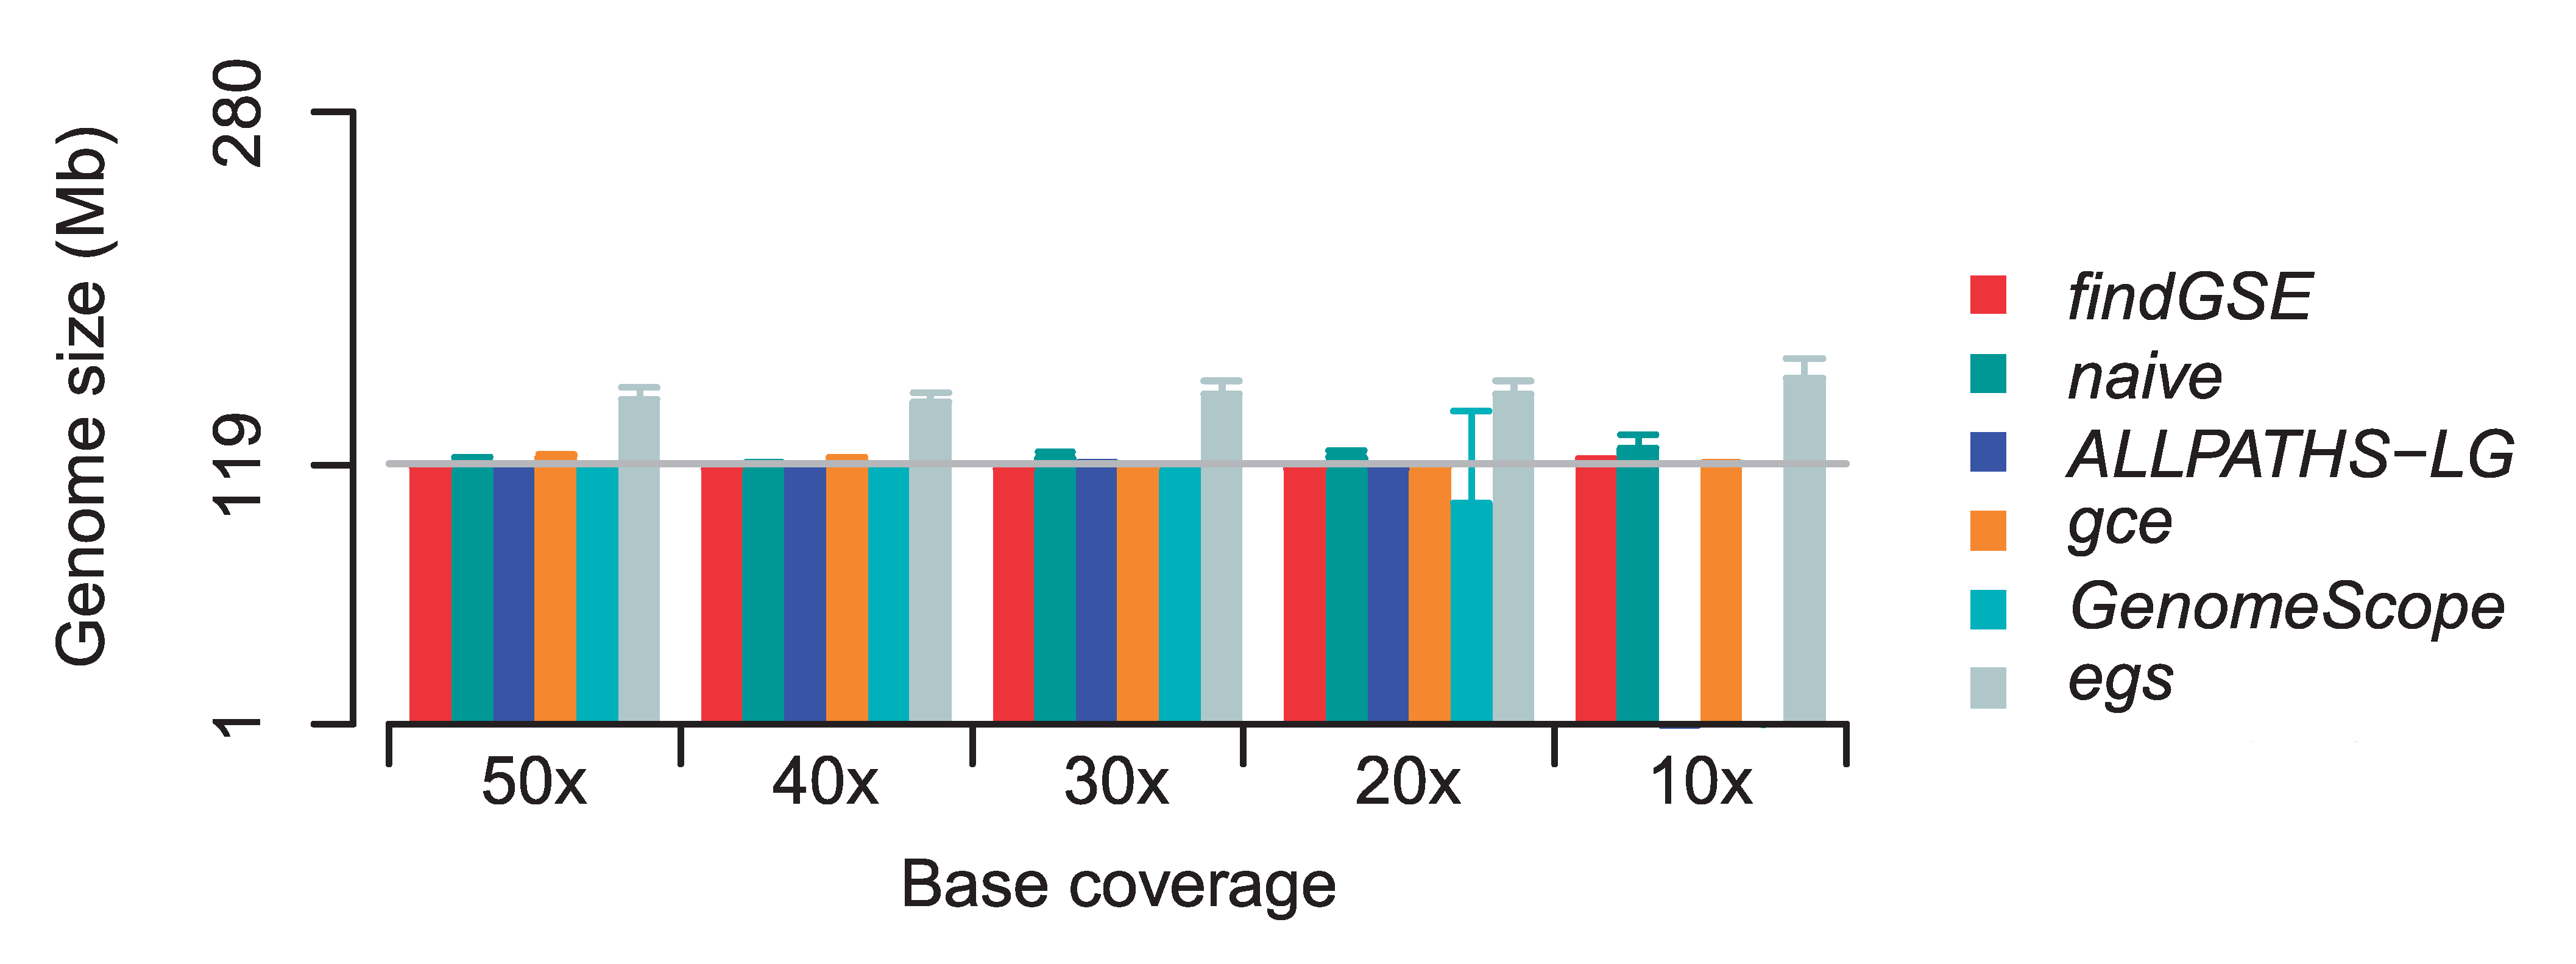
\includegraphics[height=0.21\textheight]{capitoli/analisi/confronto/confronto1/a.png}
		\caption{Stima della dimensione del genoma, con valore di copertura minima variabile.}
		\label{fig:confronto1}
	\end{figure}

	\paragraph{Errori di sequenziamento}
	Modificando invece il rapporto di errore di sequenziamento, i programmi generano risultati quasi sempre compatibili con la grandezza reale, come mostrato dalla figura~\vref{fig:confronto2}. Si noti che con un rapporto di errore elevato e non realistico (5\%), mentre gli altri metodi mantengono la stessa precisione ALLPATHS-LG restituisce un valore instabile.
	
	\begin{figure}
		\centering
		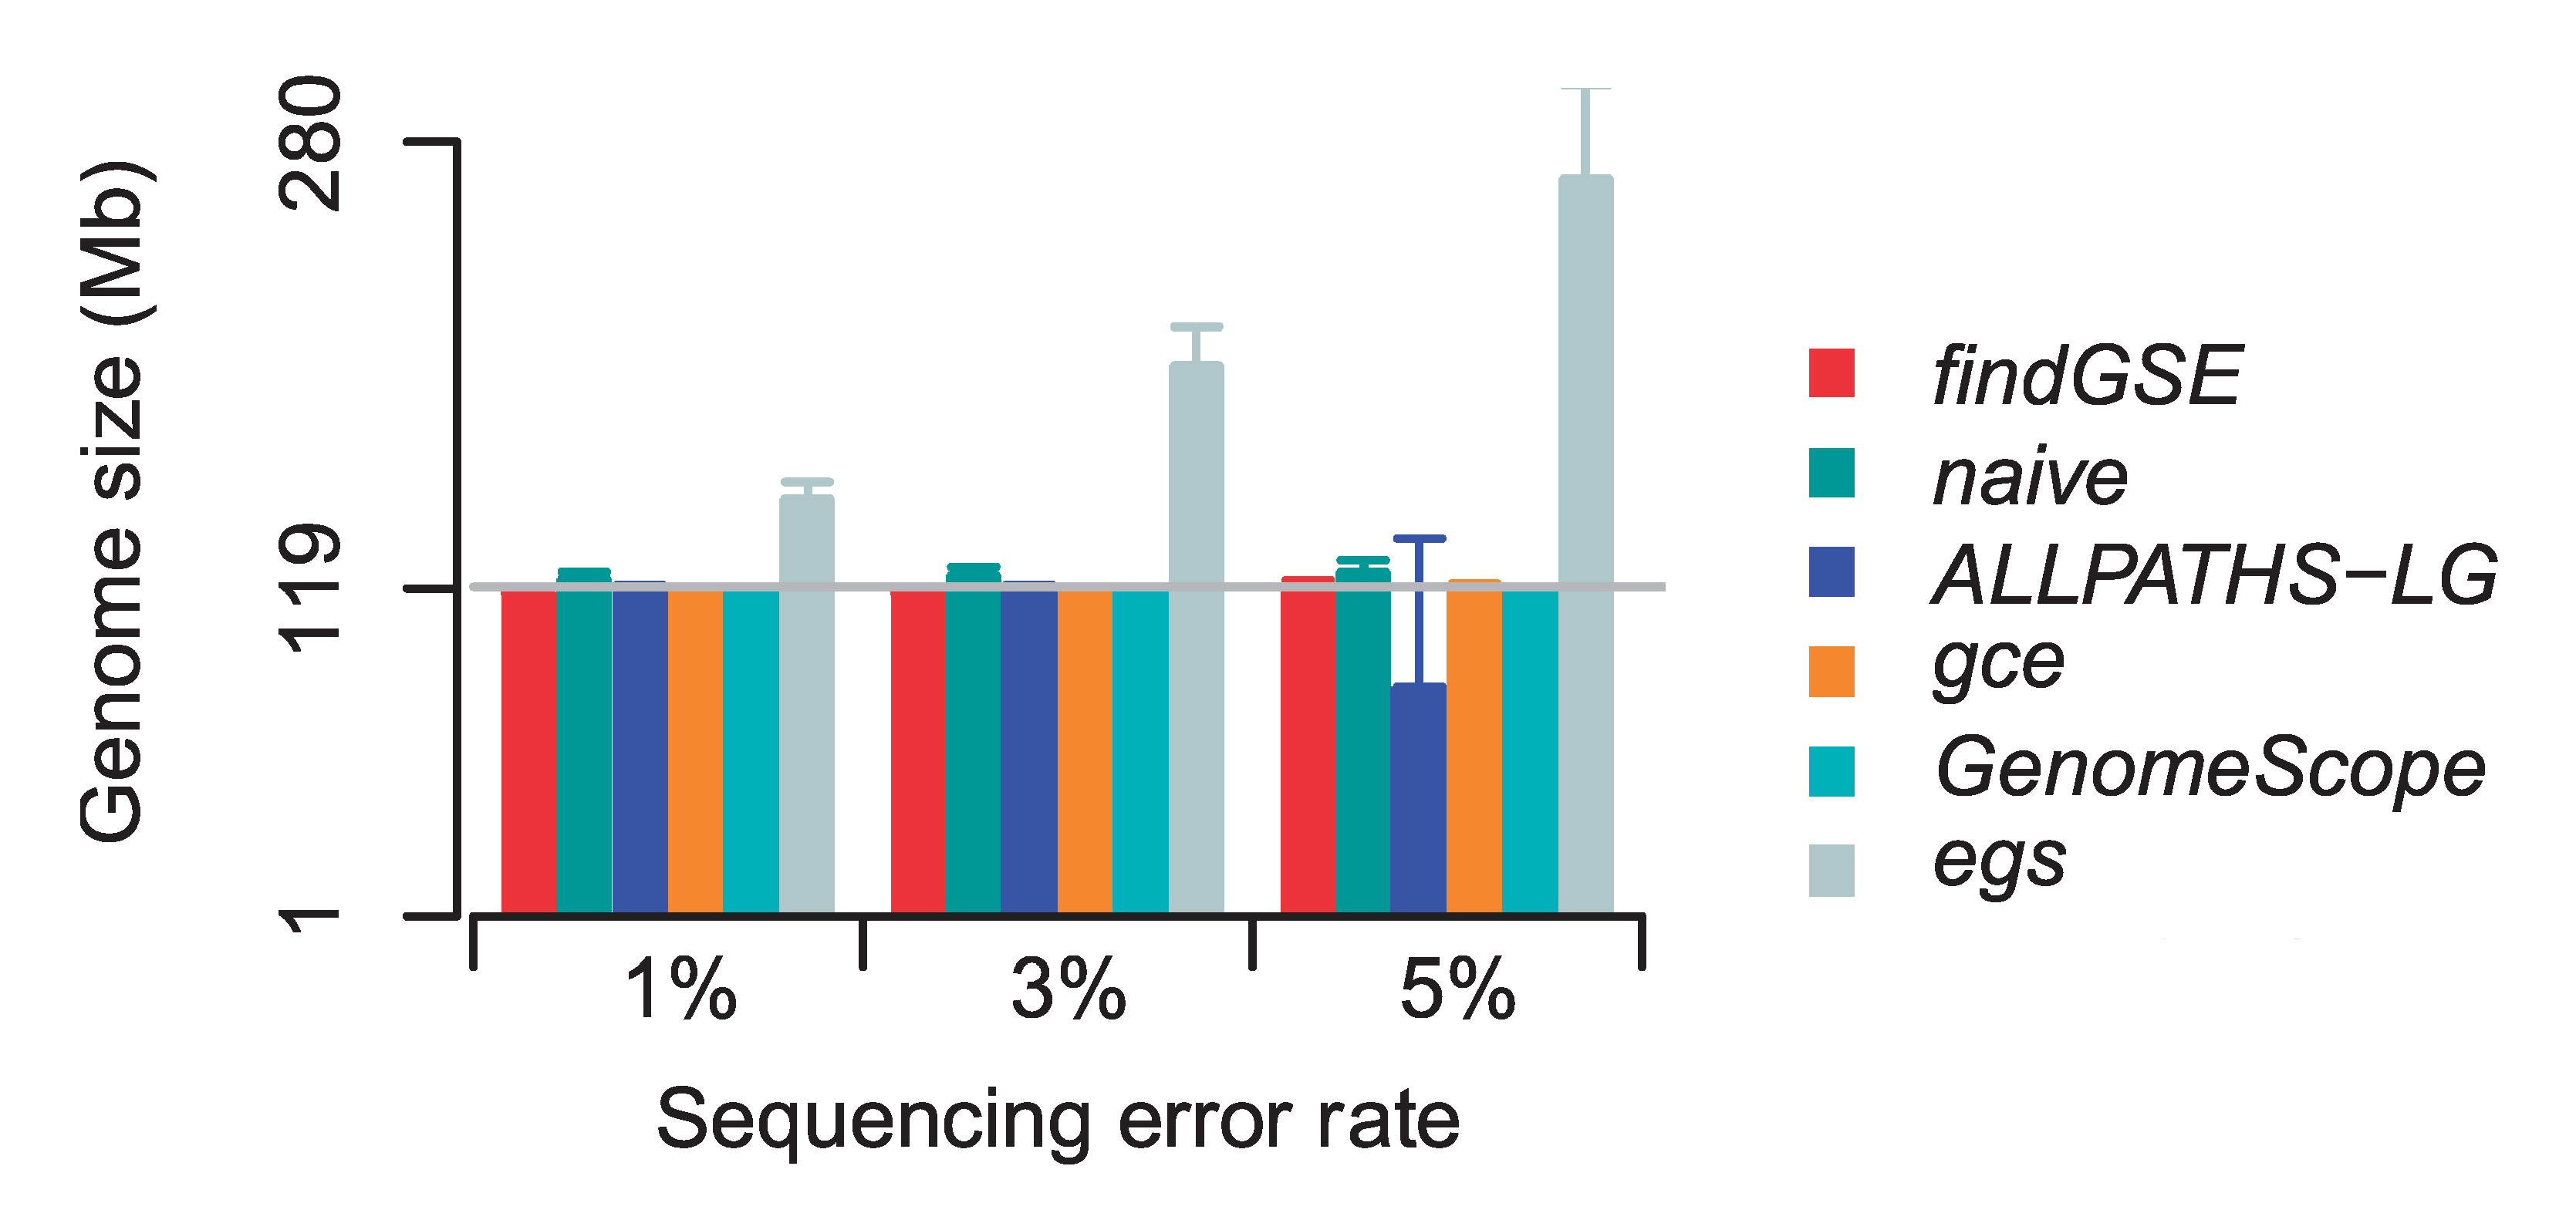
\includegraphics[height=0.21\textheight]{capitoli/analisi/confronto/confronto1/c.png}
		\caption{Stima della dimensione del genoma con tasso di errore di sequenziamento variabile.}
		\label{fig:confronto2}
	\end{figure}

	\paragraph{Influenza dell'eterozigosi}
	Per la valutazione dell'impatto dell'eterozigosi, è stata considerata una sequenza con copertura 30$\times$, un rapporto di errore di sequenziamento dell'1\% e un rapporto di mutazioni \gls{snp} da 0,1 a 5,0\%. Per livelli bassi di eterozigosi (da 0,1 a 1,0\%) tutti i metodi risultano precisi e concordi, come mostrato dalla figura~\ref{fig:confronto3}. 
	
	Aumentando il \gls{rate_eterozigosity} (da 2,0 a 5,0\%), la discrepanza tra i valori predetti e quello reale aumenta considerevolmente: su un totale di 280 stime per metodo infatti, i programmi ALLPATHS-LG e GenomeScope hanno generato valori doppi rispetto alla grandezza reale rispettivamente in 150 e 29 previsioni. Le stime erronee dei due programmi sono dovute all'erronea selezione del picco eterozigote come se fosse quello omozigote, che porta a un calcolo non corretto della copertura e quindi al raddoppio della dimensione totale stimata. Gli stessi metodi hanno riportato valori nulli o estremamente bassi rispettivamente in 110 e 173 casi, generando quindi in totale valori erronei con probabilità del 92,9\% per \mbox{ALLPATHS-LG} e del 72,1\% per \mbox{GenomeScope}. 
	Anche nel caso del metodo GCE, un alto tasso di eterozigosi fa generare al programma 120 valori errati su 280 totali, cioè nel 42,9\% delle predizioni. 
	Il metodo findGSE si dimostra poco influenzato dall'aumento del \gls{rate_eterozigosity}, che nel peggiore dei casi fa sovrastimare di poco la dimensione del genoma \mbox{(125 $\pm$ 7 Mb)}.
 
 	\begin{figure}
 		\centering
 		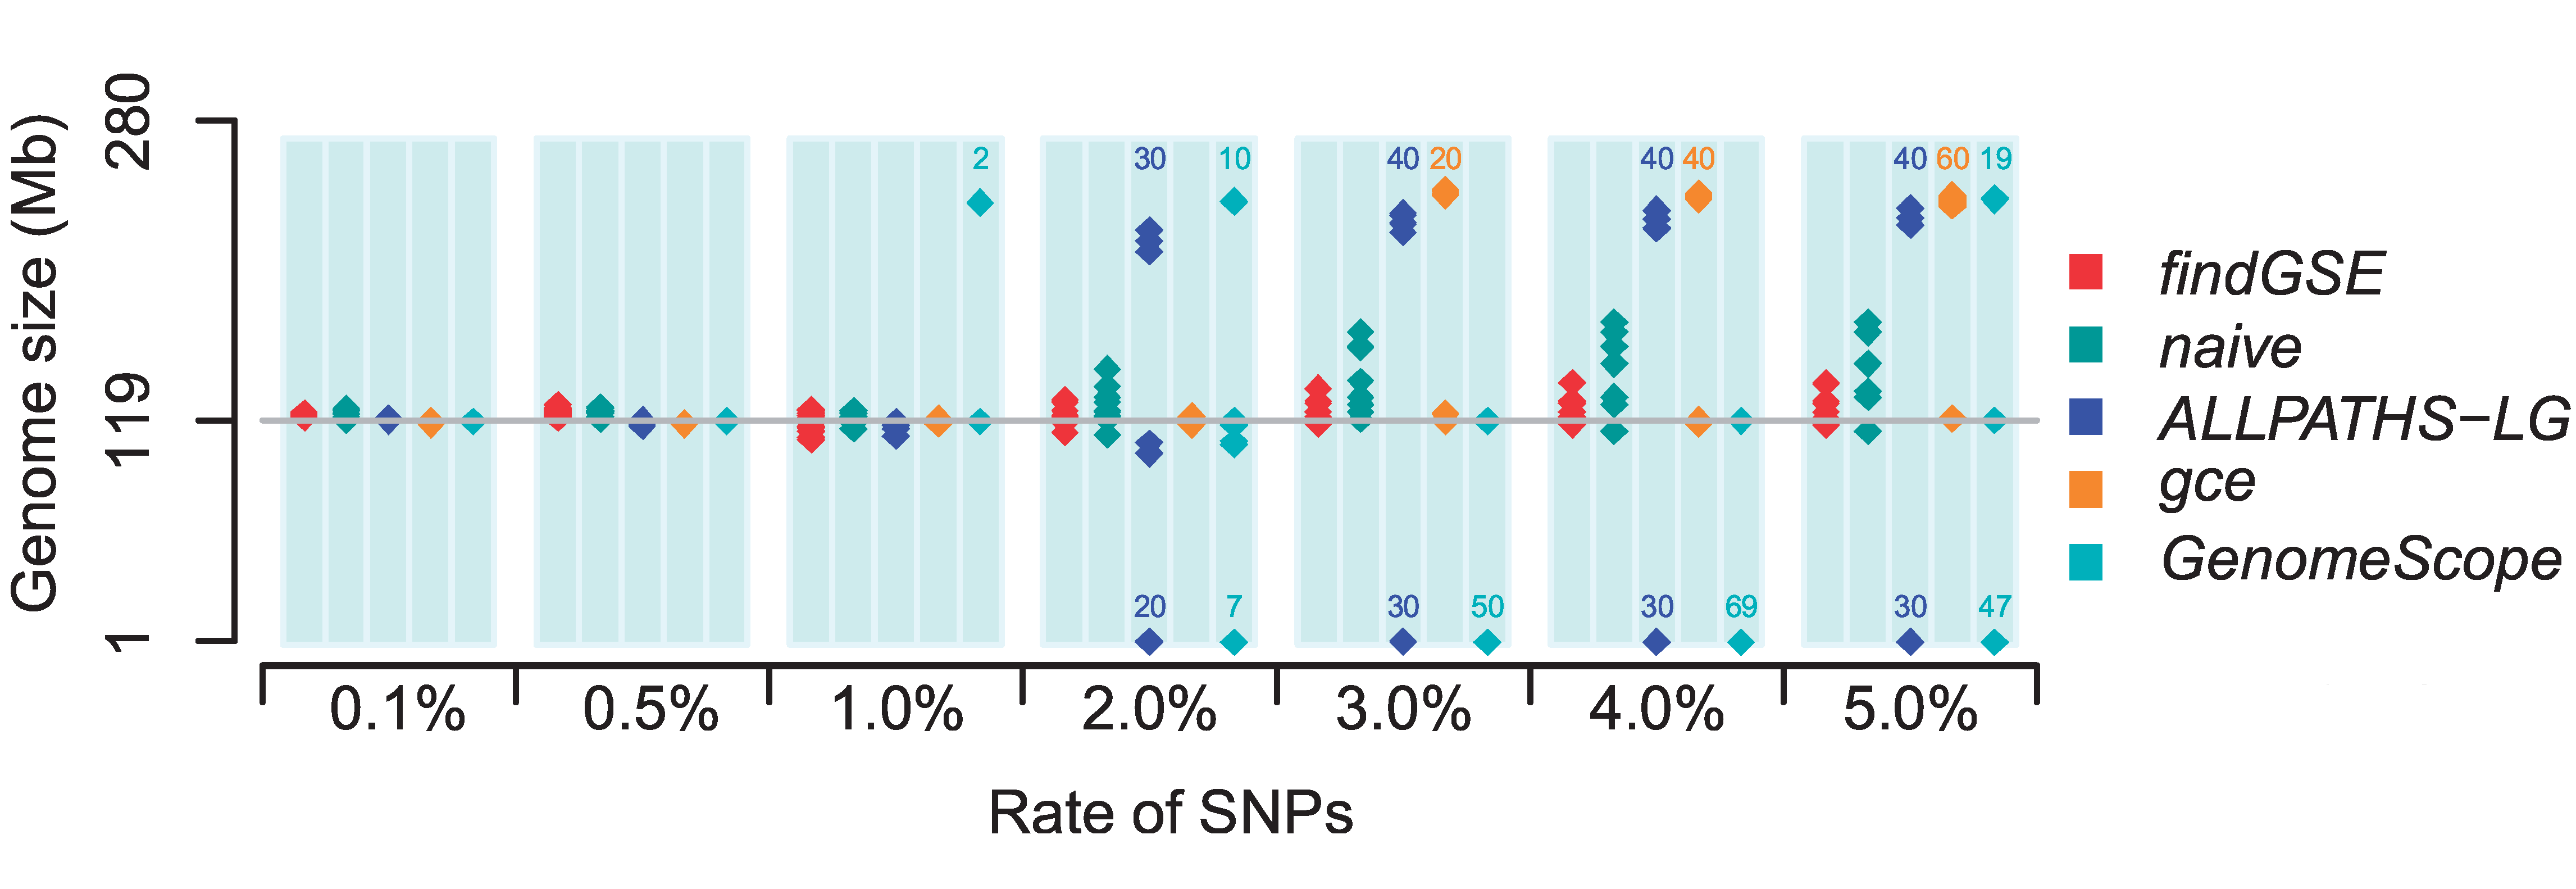
\includegraphics[height=0.21\textheight]{capitoli/analisi/confronto/confronto1/d.png}
 		\caption{Stima della dimensione del genoma con livello di eterozigosi variabile e copertura base 30$\times$. Si noti che i valori rappresentati indicano il numero di punti sovrapposti in una certa regione.}
 		\label{fig:confronto3}
 	\end{figure}
 
 	Mantenendo elevato il tasso di errore di sequenziamento, l'aumento della copertura minima a 100$\times$ (figura~\ref{fig:confronto4}) diminuisce il numero di stime non corrette per i metodi ALLPATHS-LG e GenomeScope, generando rispettivamente 60 (21,4\%) e 110 (39,3\%) valori errati. 
 	Il programma GCE invece, anche all'aumentare della copertura produce molti risultati errati, 210 su 280 totali (75\%).
 	Il metodo findGSE infine si dimostra molto accurato anche ad un alto \gls{rate_eterozigosity}, stimando una dimensione media di \mbox{121 $\pm$ 1 Mb}. 
 	Il programma GenomeScope, tralasciando il problema di duplicazione della dimensione, si dimostra quello con i risultati più stabili tra i  metodi analizzati.
 	
	 \begin{figure} 
	 	\centering
	 	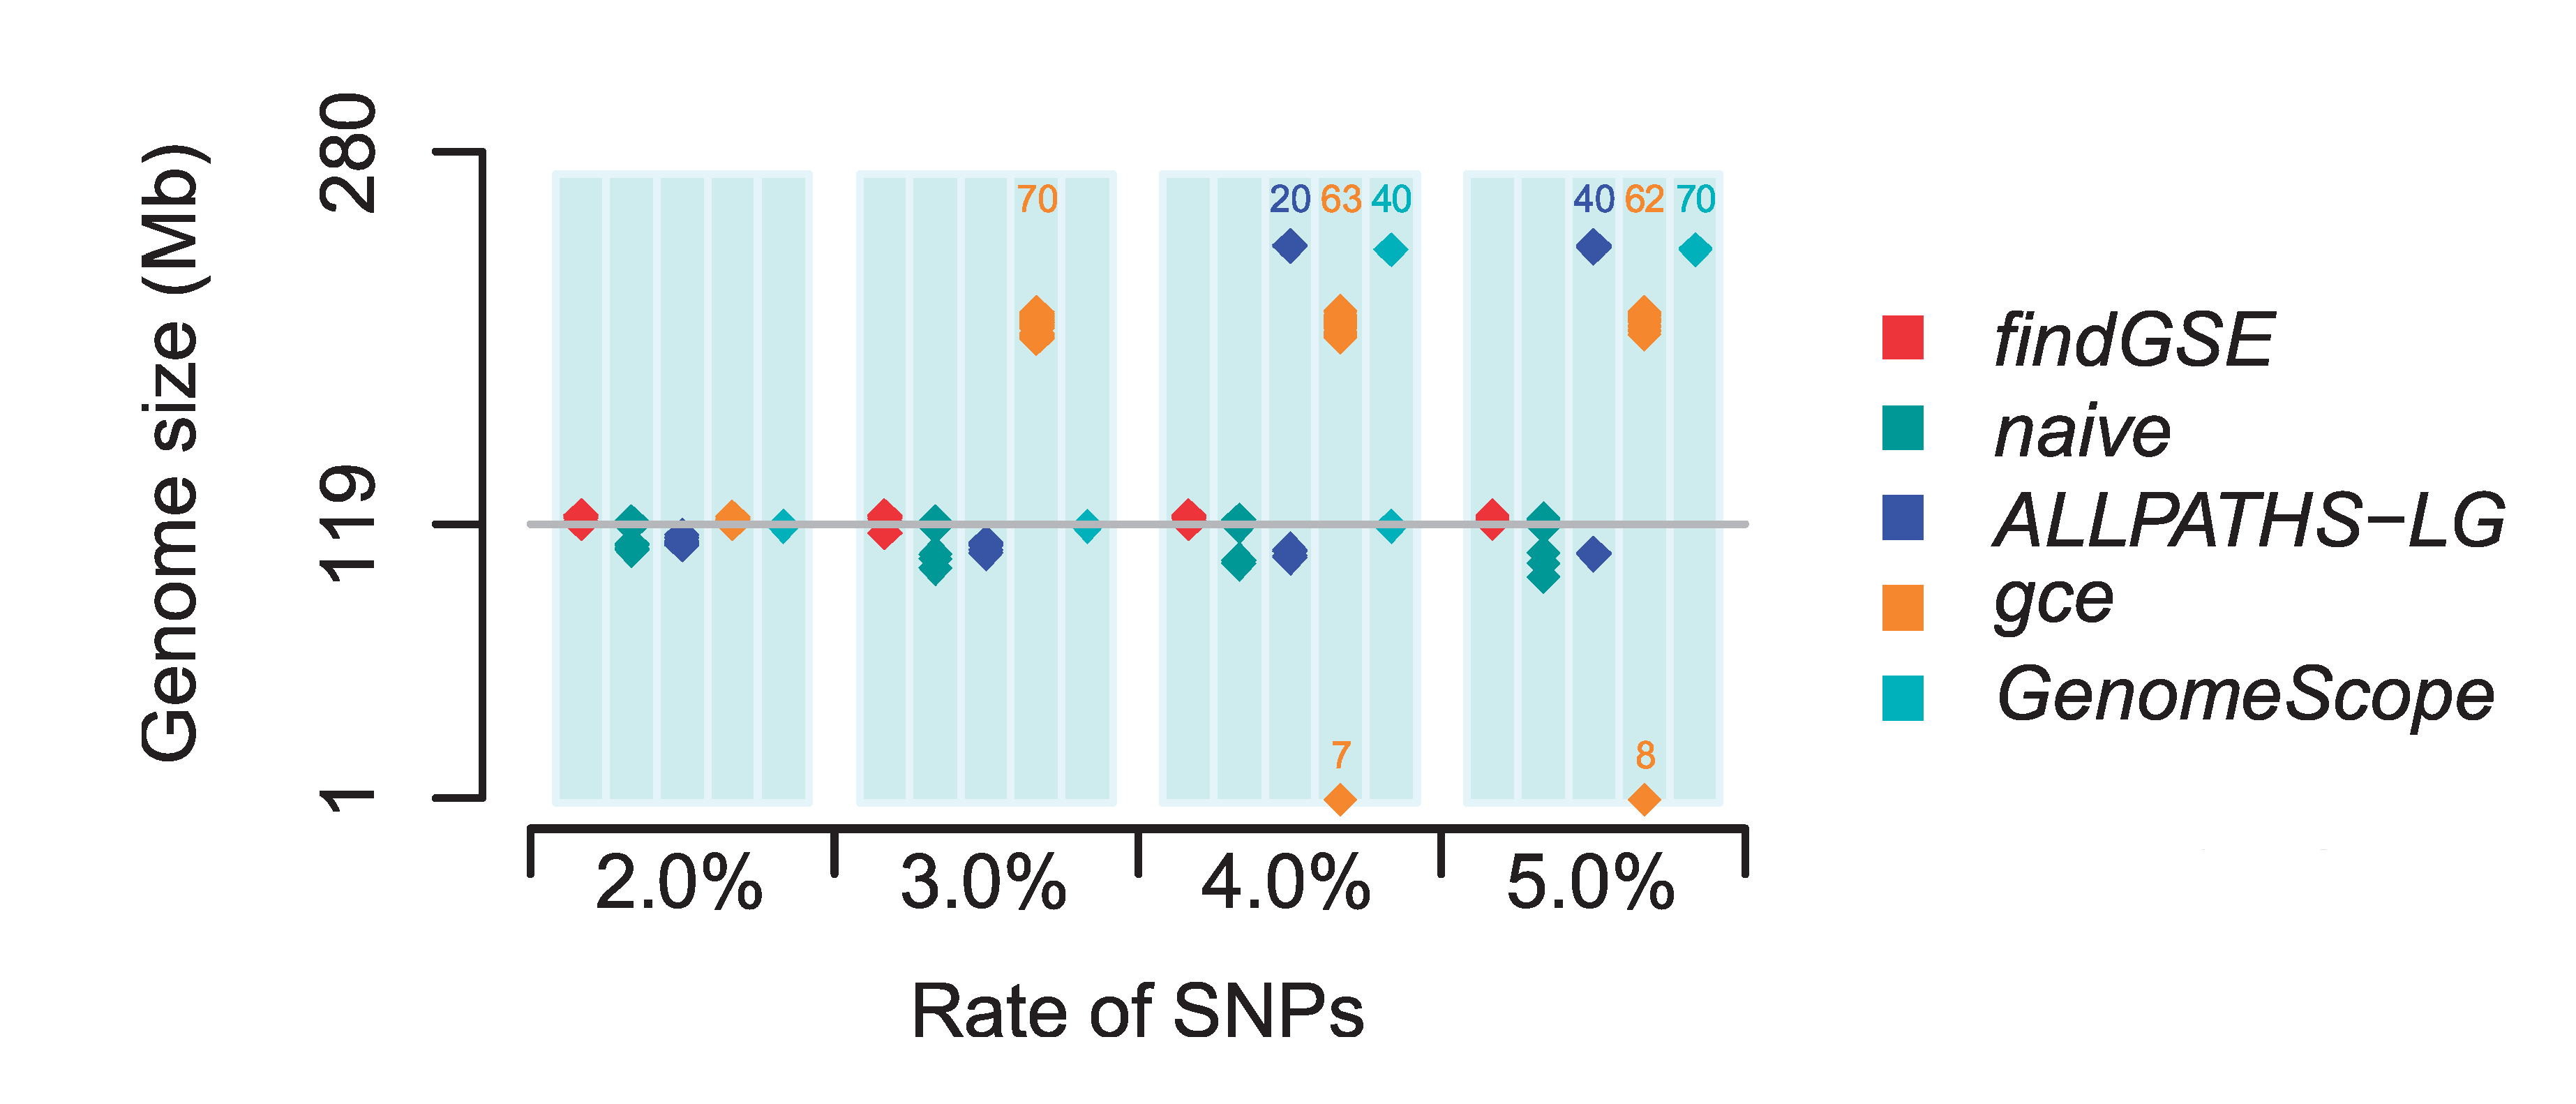
\includegraphics[height=0.21\textheight]{capitoli/analisi/confronto/confronto1/e.png}
	 	\caption{Stima della dimensione del genoma con livello di eterozigosi variabile e copertura base 100$\times$. Si noti che i valori rappresentati indicano il numero di punti sovrapposti in una certa regione.}
	 	\label{fig:confronto4}
	 \end{figure}
 
 	\paragraph{Stima di sequenze reali}
 	La riproducibilità dei metodi analizzati è stata verificata con la stima della dimensione di sette genomi reali. Le sequenze scelte per la verifica sono sequenziamenti di \textit{Arabidopsis thaliana}, le cui differenze si assume non vadano a modificare considerevolmente la dimensione del genoma. La deviazione standard delle stime per ciascun metodo si presenta bassa, variando tra 2 Mb (findGSE) e 5 Mb (GCE), come mostra la figura~\vref{fig:confronto5a}. Ciò può dimostrare la robustezza dei programmi rispetto ad eventuali variazioni nel sequenziamento del genoma, e l'alta riproducibilità che li caratterizza.

 	Per verificare l'indipendenza tra il valore stimato e la copertura di letture reali, i metodi sono stati utilizzati per stimare la dimensione del genoma di \textit{A. thaliana} a partire da 89 sequenze con copertura base minima maggiore di 19$\times$. Come mostra la figura~\vref{fig:confronto5b}, le stime di ciascun programma risultano indipendenti da tale valore.
 	
 	\begin{figure}[p]
 		\centering
 		\subfloat[][\emph{Valori stimati, media e deviazione standard di ciascun metodo.}\label{fig:confronto5a}]
 			{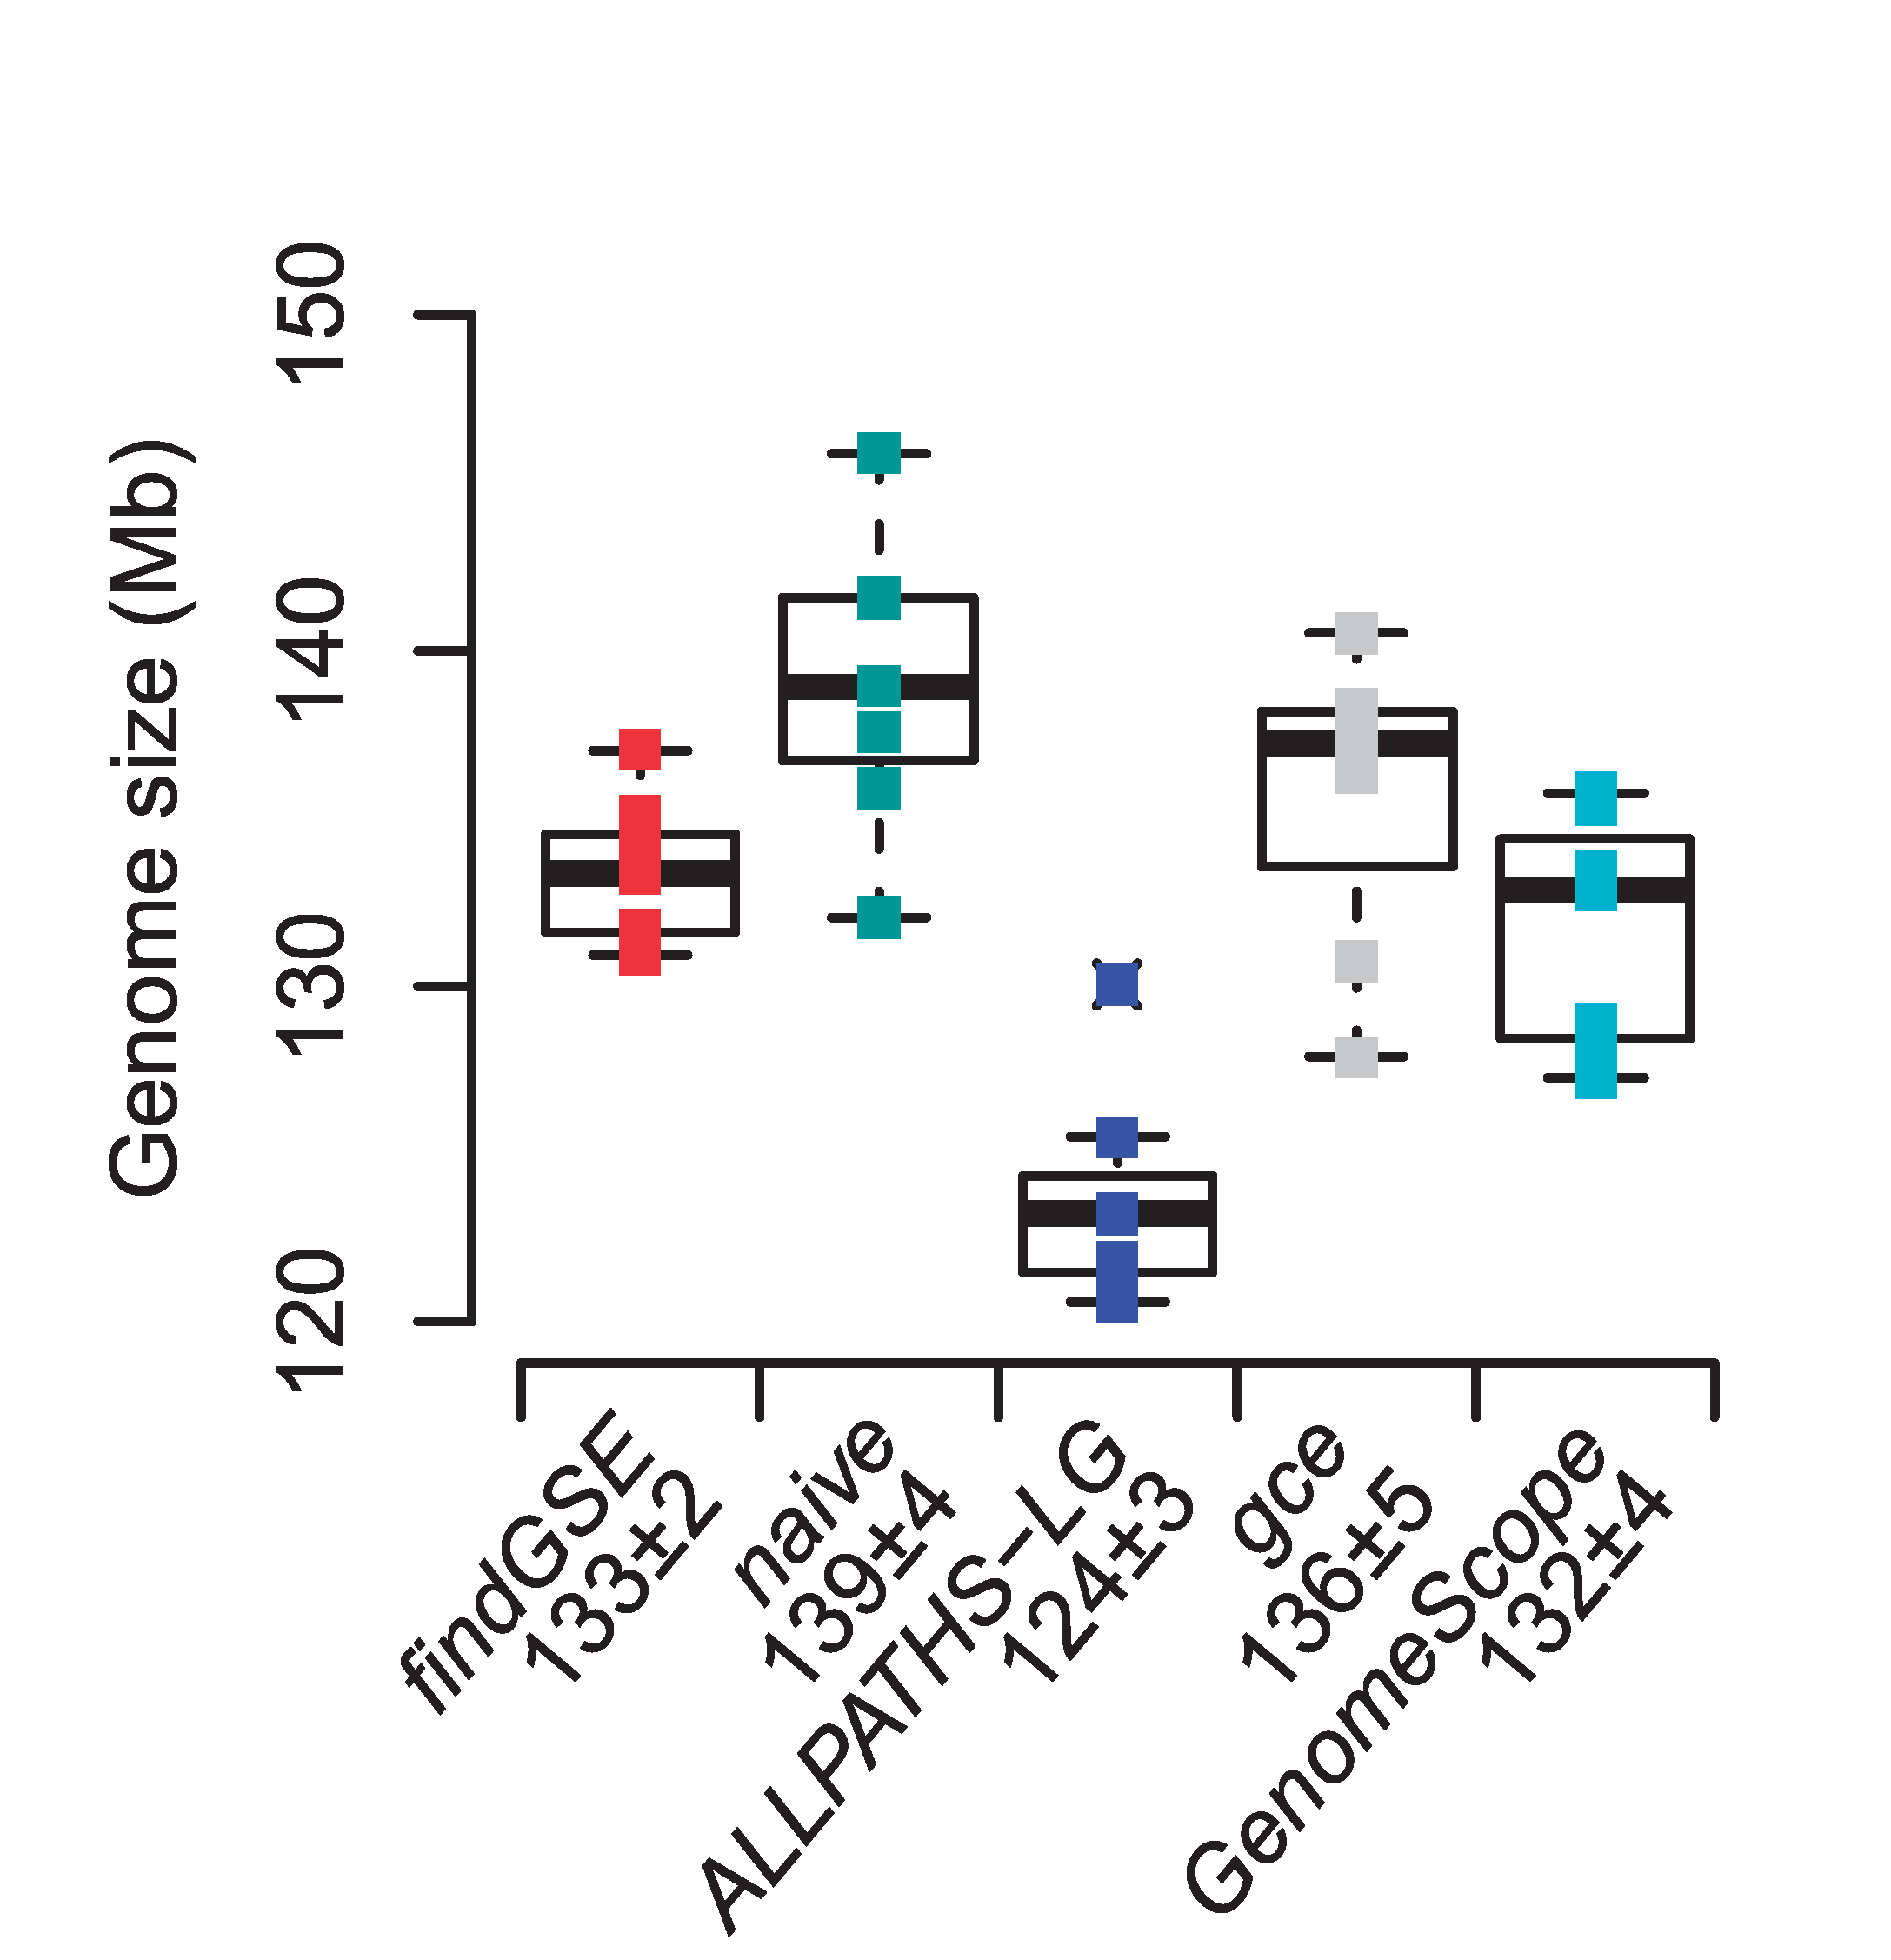
\includegraphics[width=0.37\textwidth]{capitoli/analisi/confronto/confronto1/f.png}} \qquad 
 		\subfloat[][\emph{Valori stimati da ciascun metodo in relazione alla copertura base.}\label{fig:confronto5b}]
 			{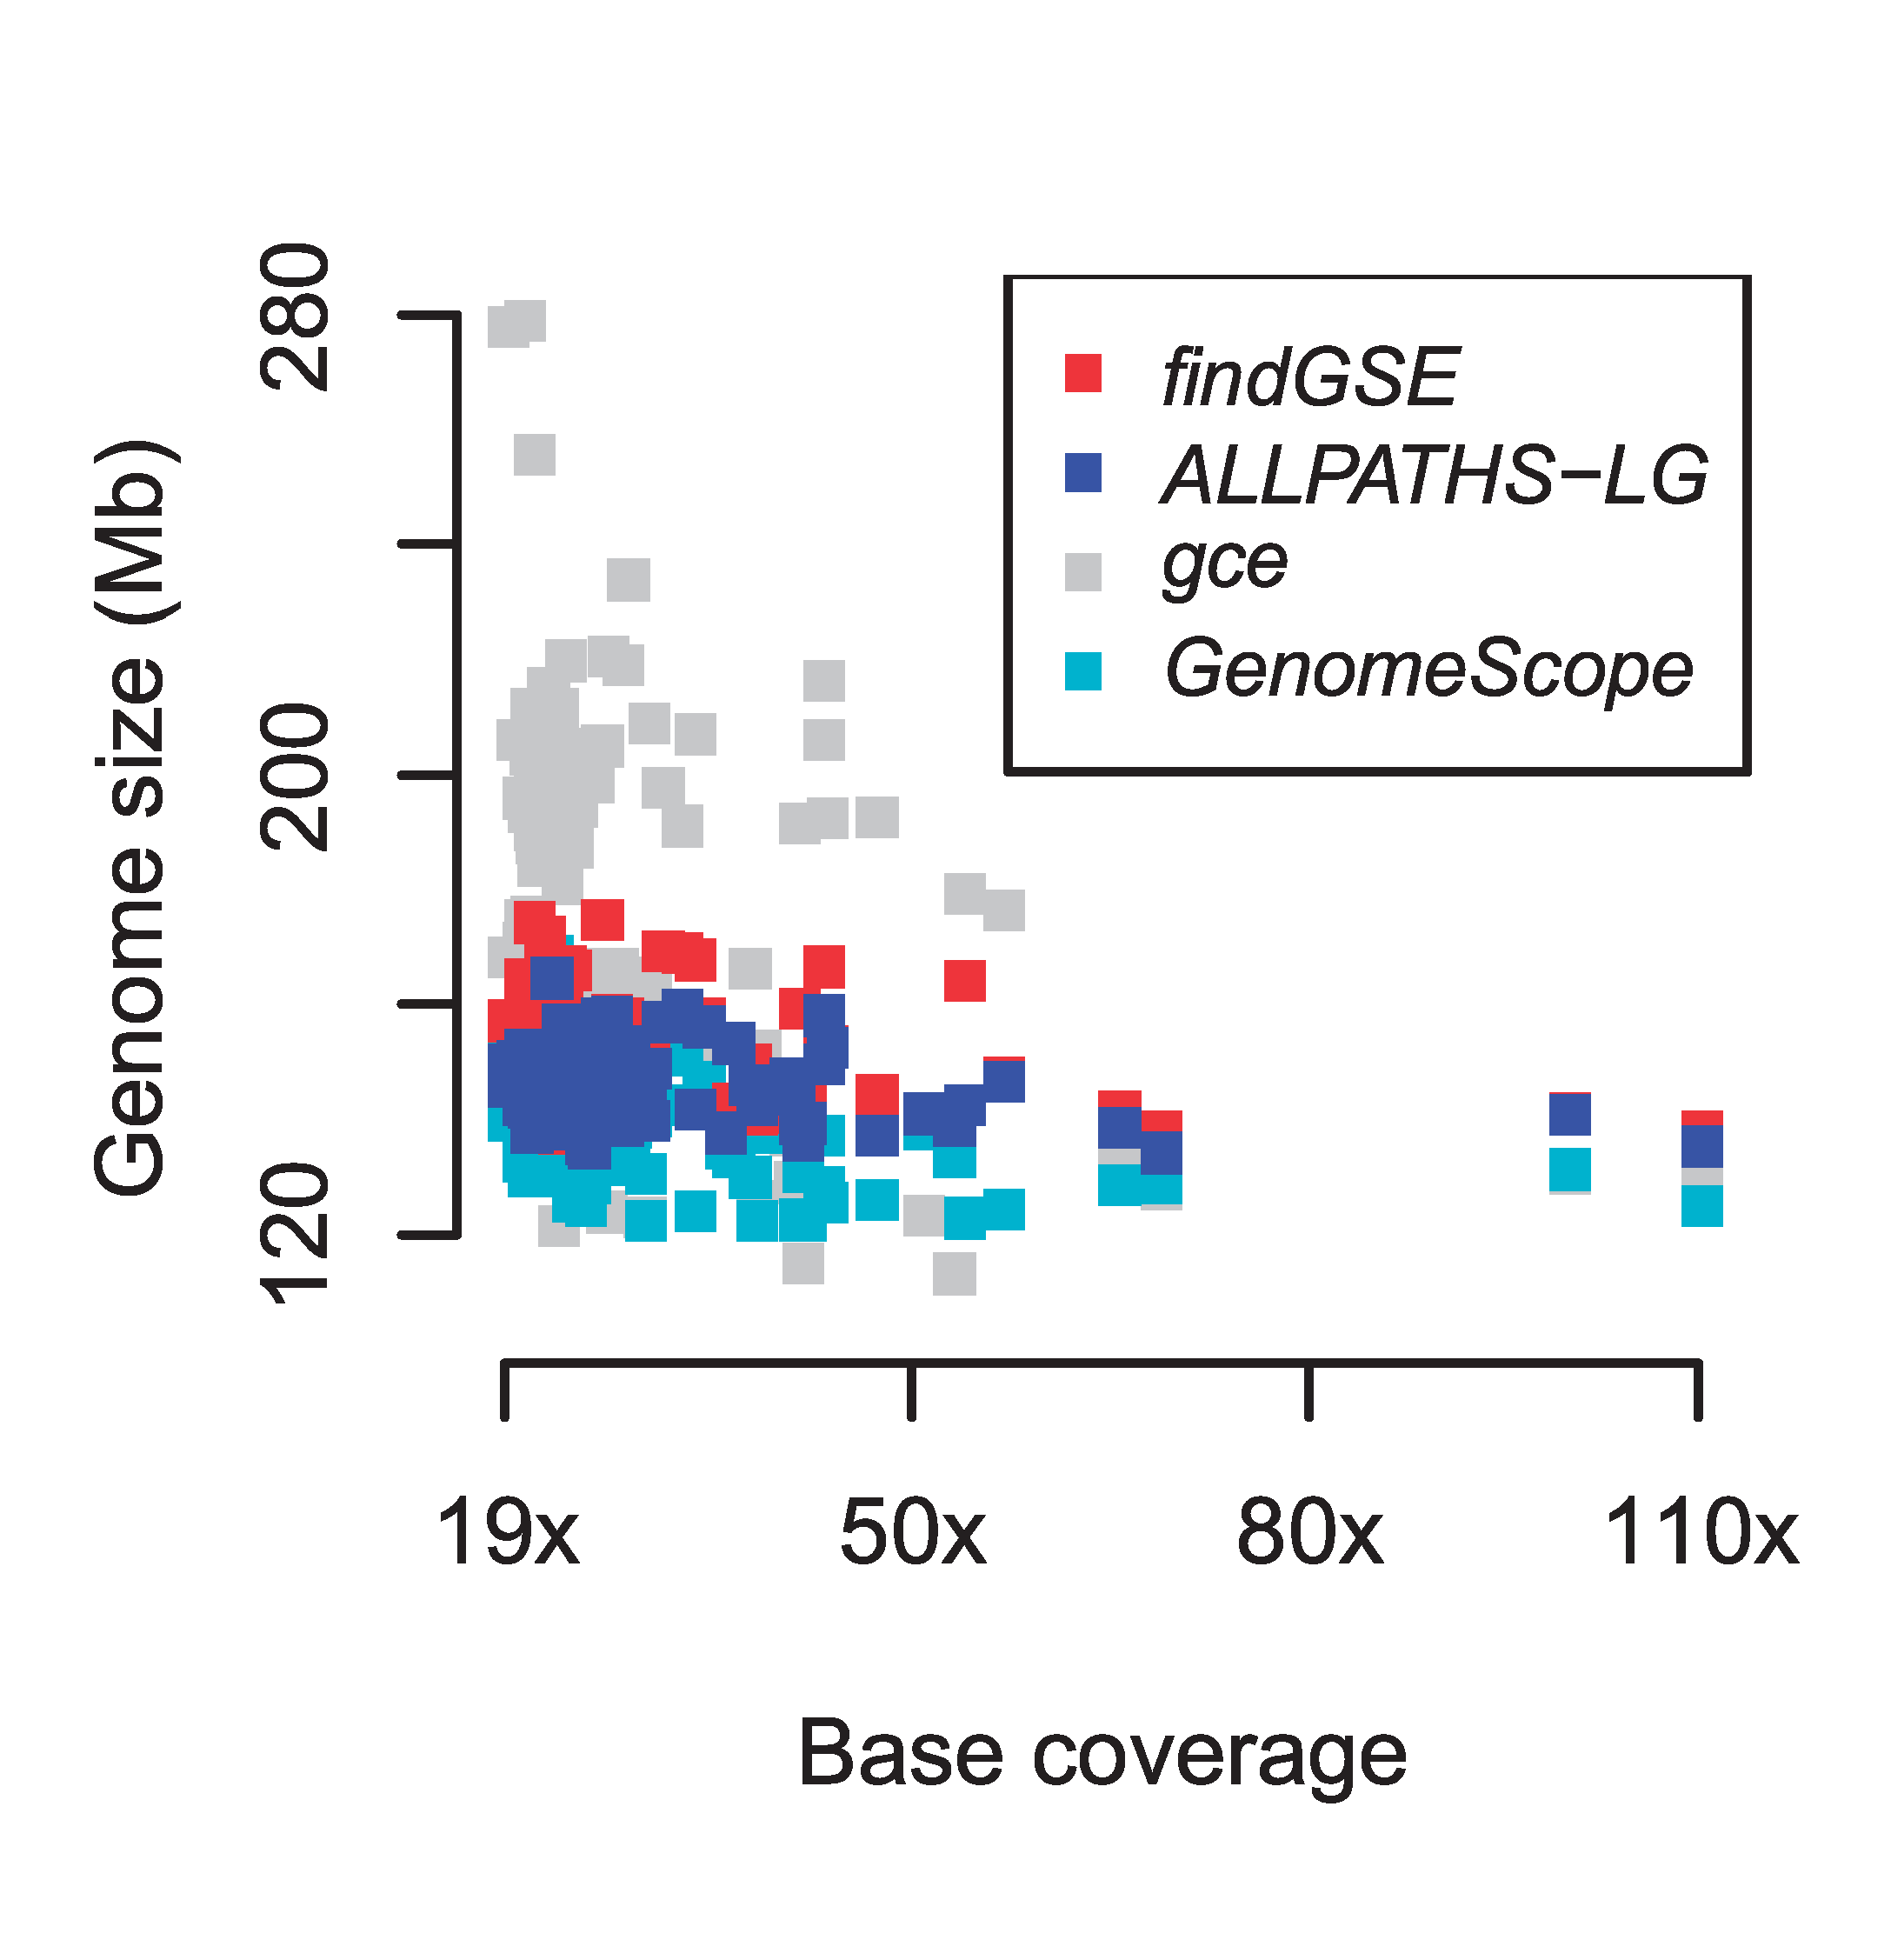
\includegraphics[width=0.37\textwidth]{capitoli/analisi/confronto/confronto1/g.png}} 
 		\caption{Confronto tra i metodi analizzati nella stima della dimensione di \textit{A. thaliana}.}
 		\label{fig:confronto5}
 	\end{figure}
 
	\paragraph{Confronto con flow cytometry}
	Sebbene il metodo flow cytometry non possa restituire una dimensione certa del genoma, è considerato un metodo sperimentale che la possa almeno approssimare. Analizzando la dimensione di 89 sequenze di \textit{A. thaliana}, la deviazione standard della stima fatta dai programmi varia tra 6 Mb e 9 Mb. Il metodo flow cytometry invece mostra una deviazione standard di 4 Mb, che suggerisce una maggior stabilità della predizione. Per ciascun programma è stato quindi misurato il \gls{pcc} con il metodo flow cytometry (figura~\vref{fig:confronto6}), assumendo che un coefficiente più alto indichi una maggior capacità di rilevare variazioni reali della dimensione del genoma. La correlazione tra findGSE e il suddetto metodo risulta la più alta ($r = $ 0,524). 
	
	I metodi findGSE, ALLPATHS-LG e GenomeScope stimano in media simili valori di dimensione (rispettivamente 152, 146 e 138 Mb), mentre GCE produce un risultato inspiegabilmente grande (177 Mb). Il valore medio stimato tramite flow cytometry invece è di 167 Mb, anche se tale metodo tende a sovrastimarne la dimensione.
	\begin{figure}[p]
		\centering
		\subfloat[][\emph{Correlazione tra i valori stimati da GCE e flow cytometry.}\label{fig:confronto6a}]
			{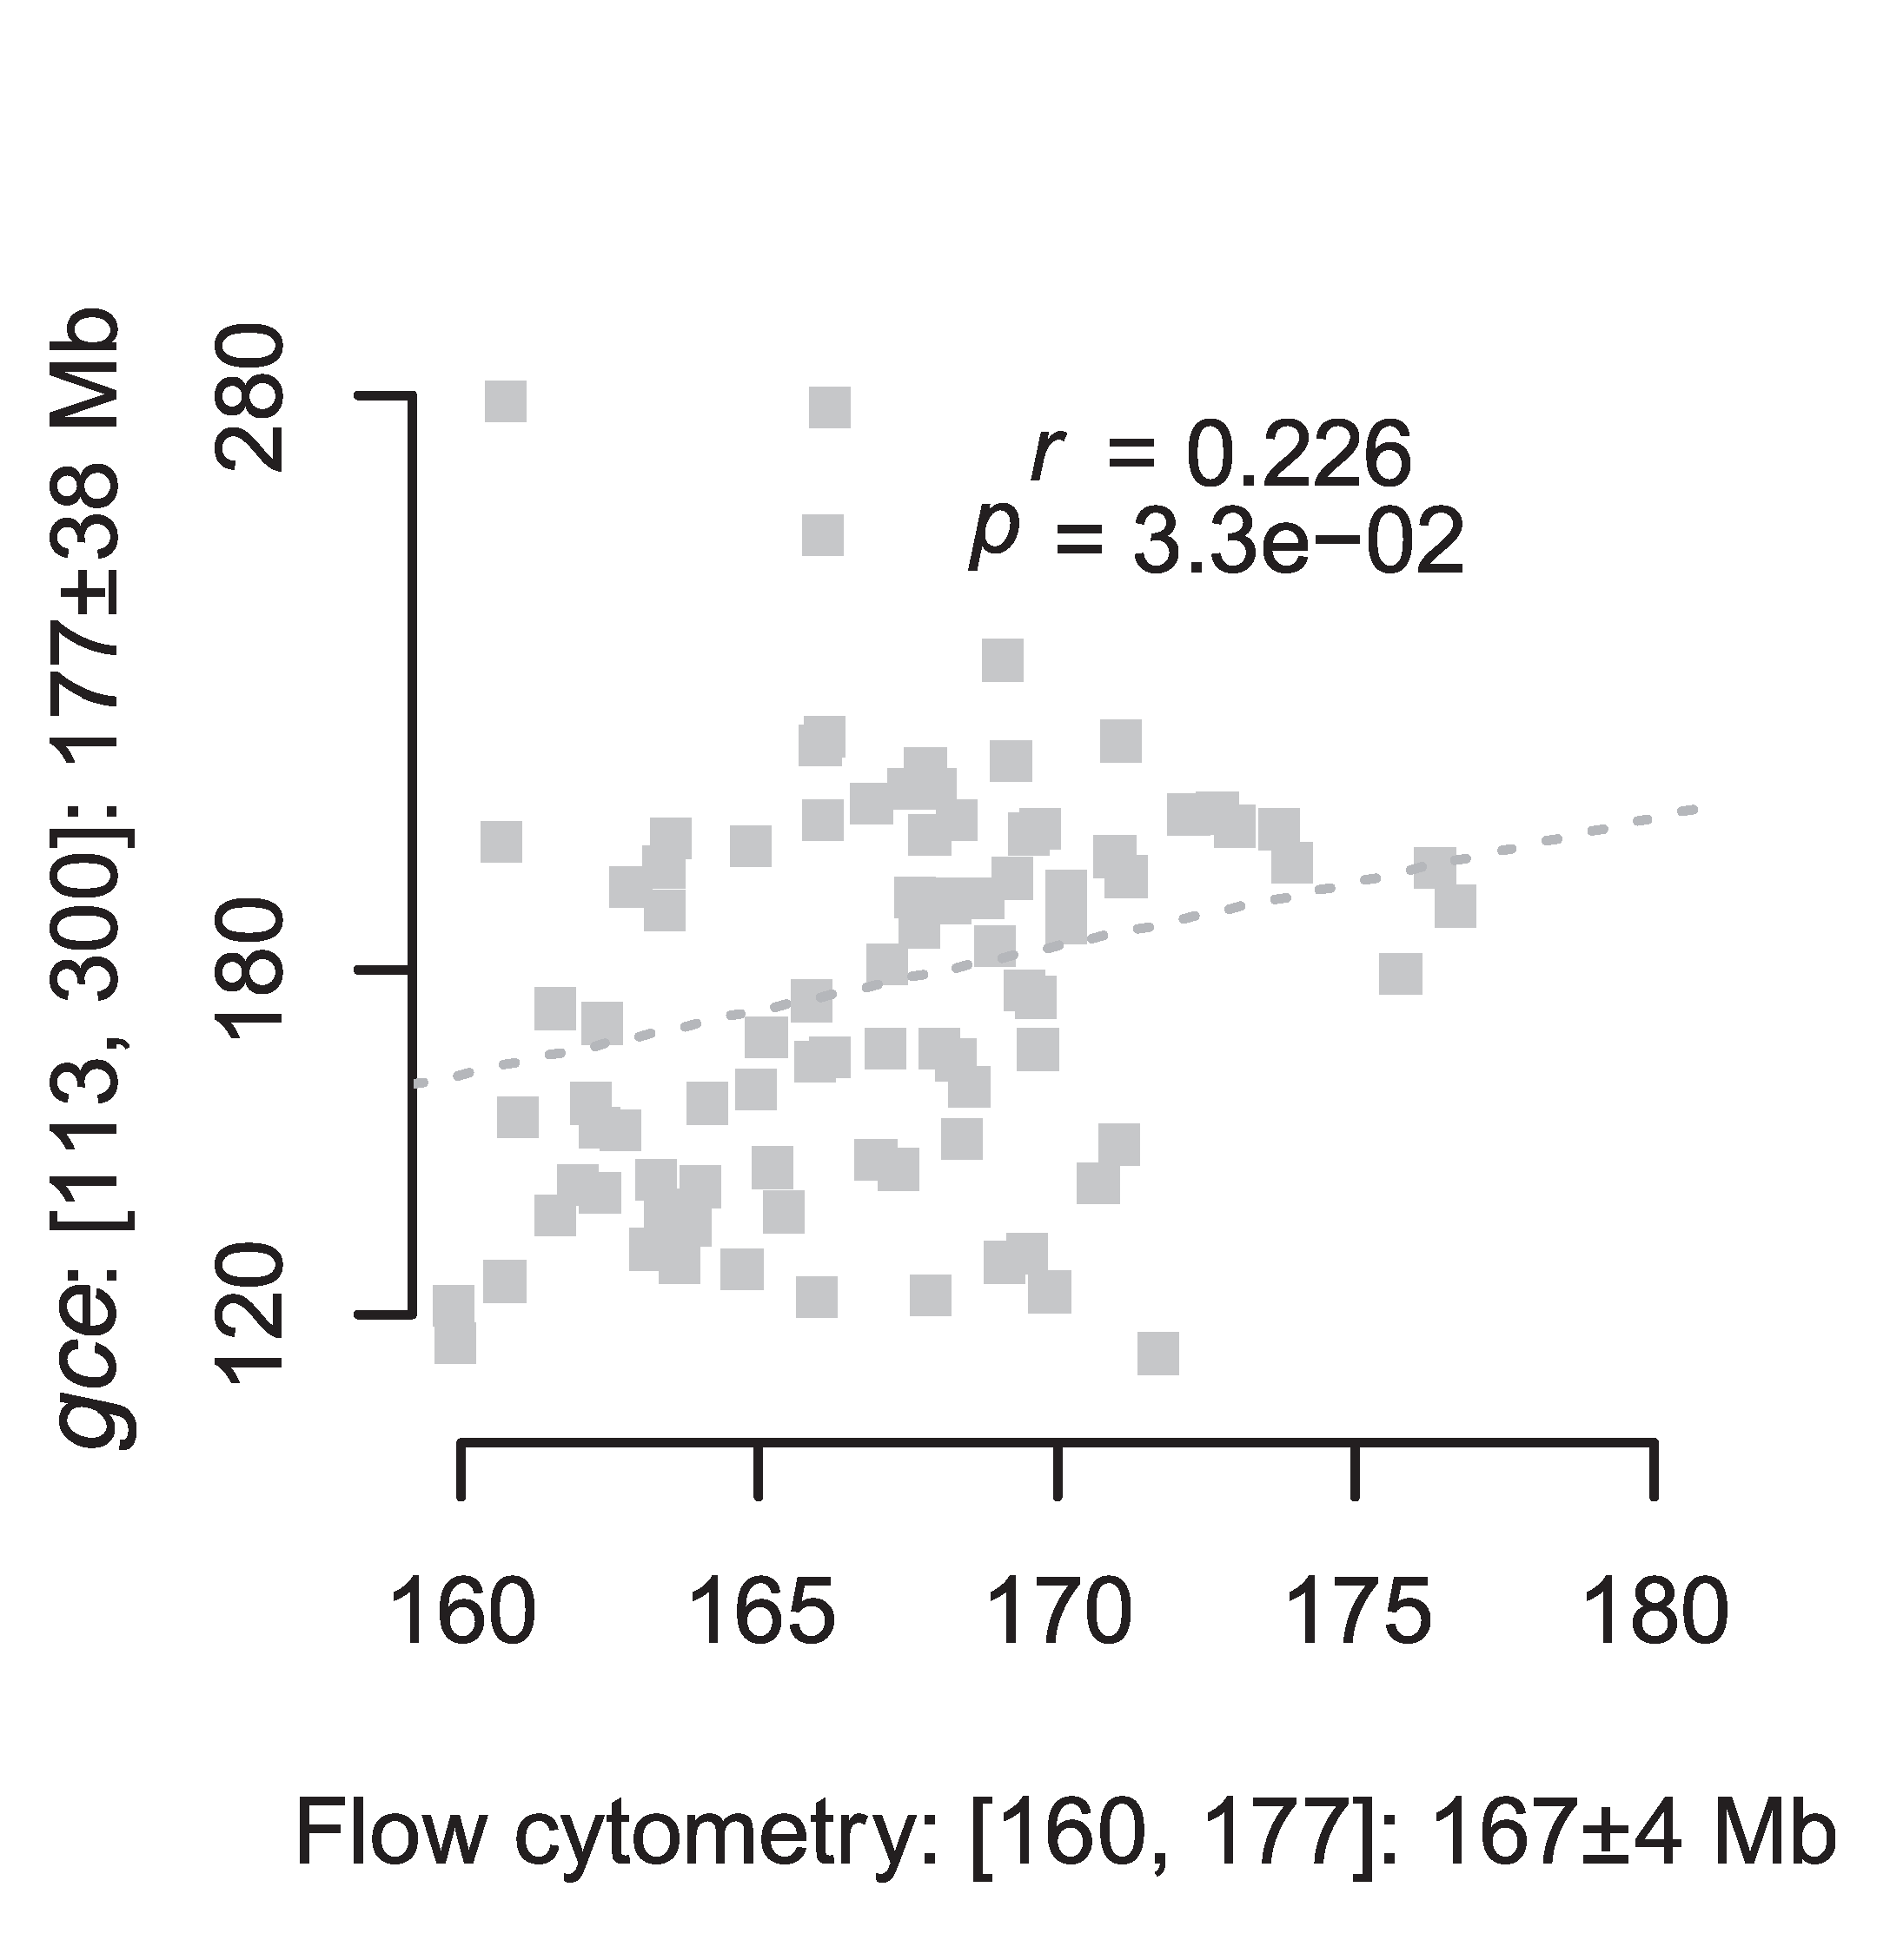
\includegraphics[width=0.37\textwidth]{capitoli/analisi/confronto/confronto1/h.png}} \qquad 
		\subfloat[][\emph{Correlazione tra i valori stimati da GenomeScope e flow cytometry.}\label{fig:confronto6b}]
			{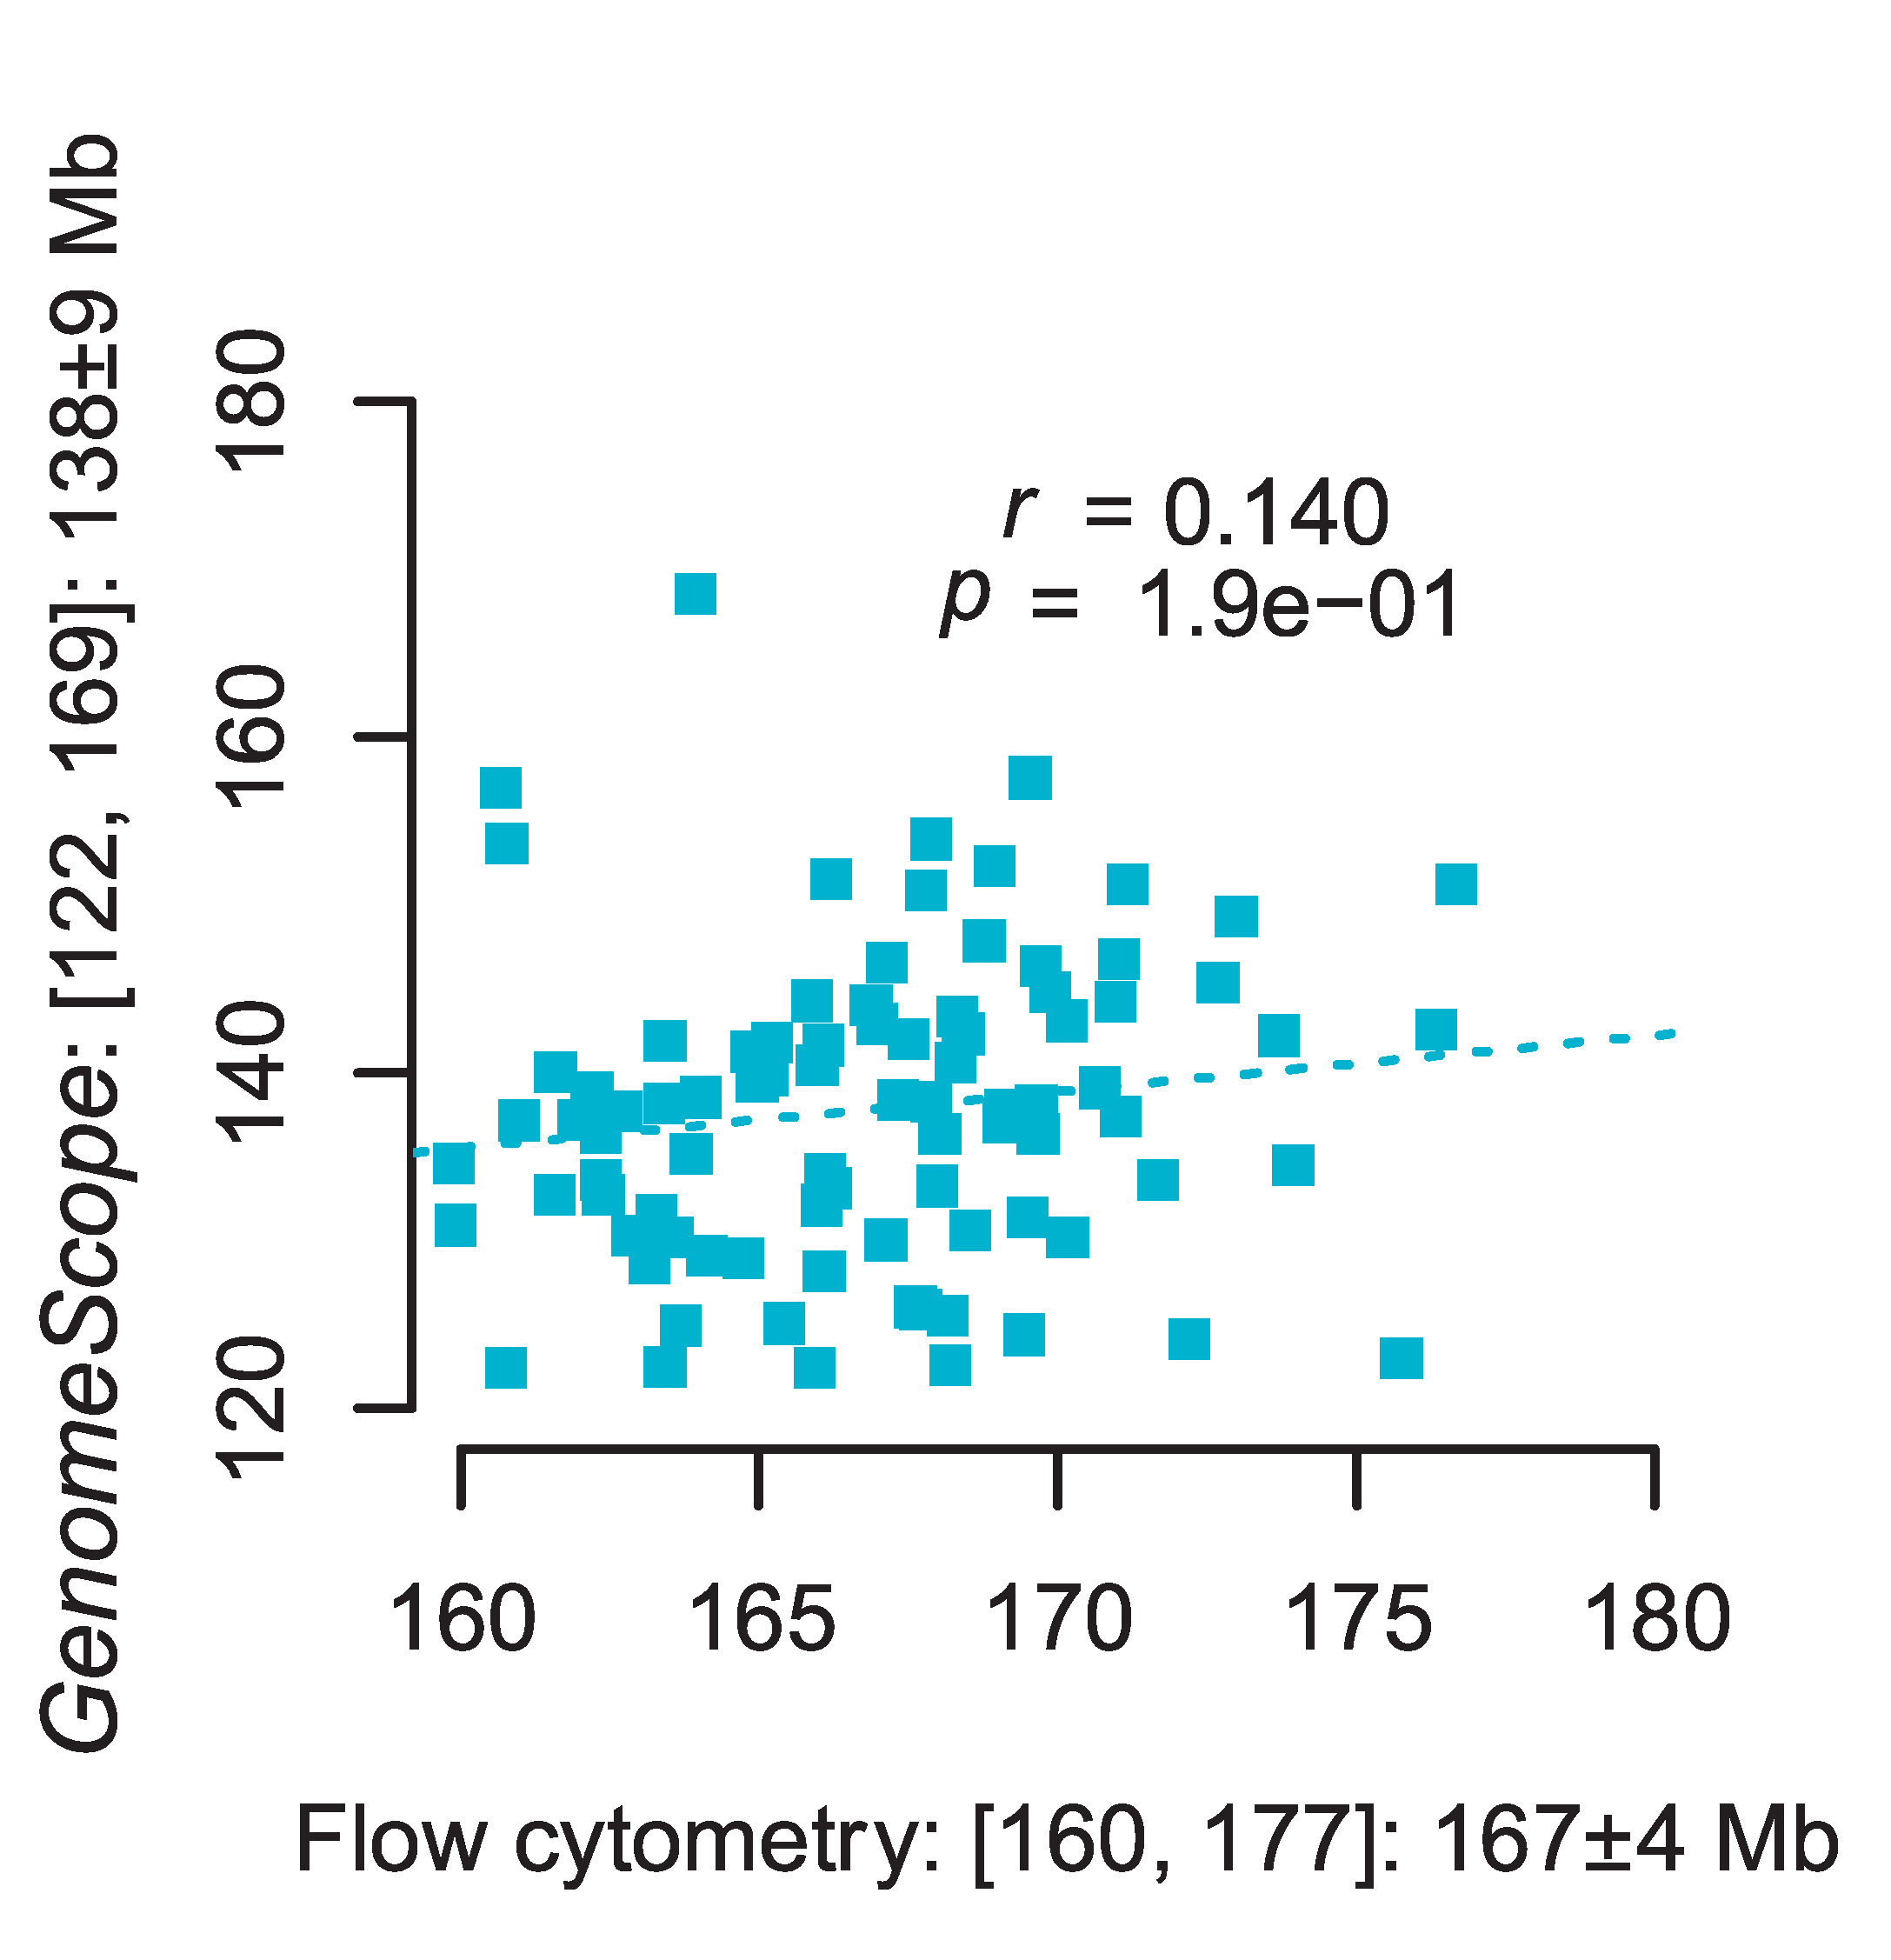
\includegraphics[width=0.37\textwidth]{capitoli/analisi/confronto/confronto1/i.png}} \\
		\subfloat[][\emph{Correlazione tra i valori stimati da ALLPATHS-LG e flow cytometry.}\label{fig:confronto6c}]
			{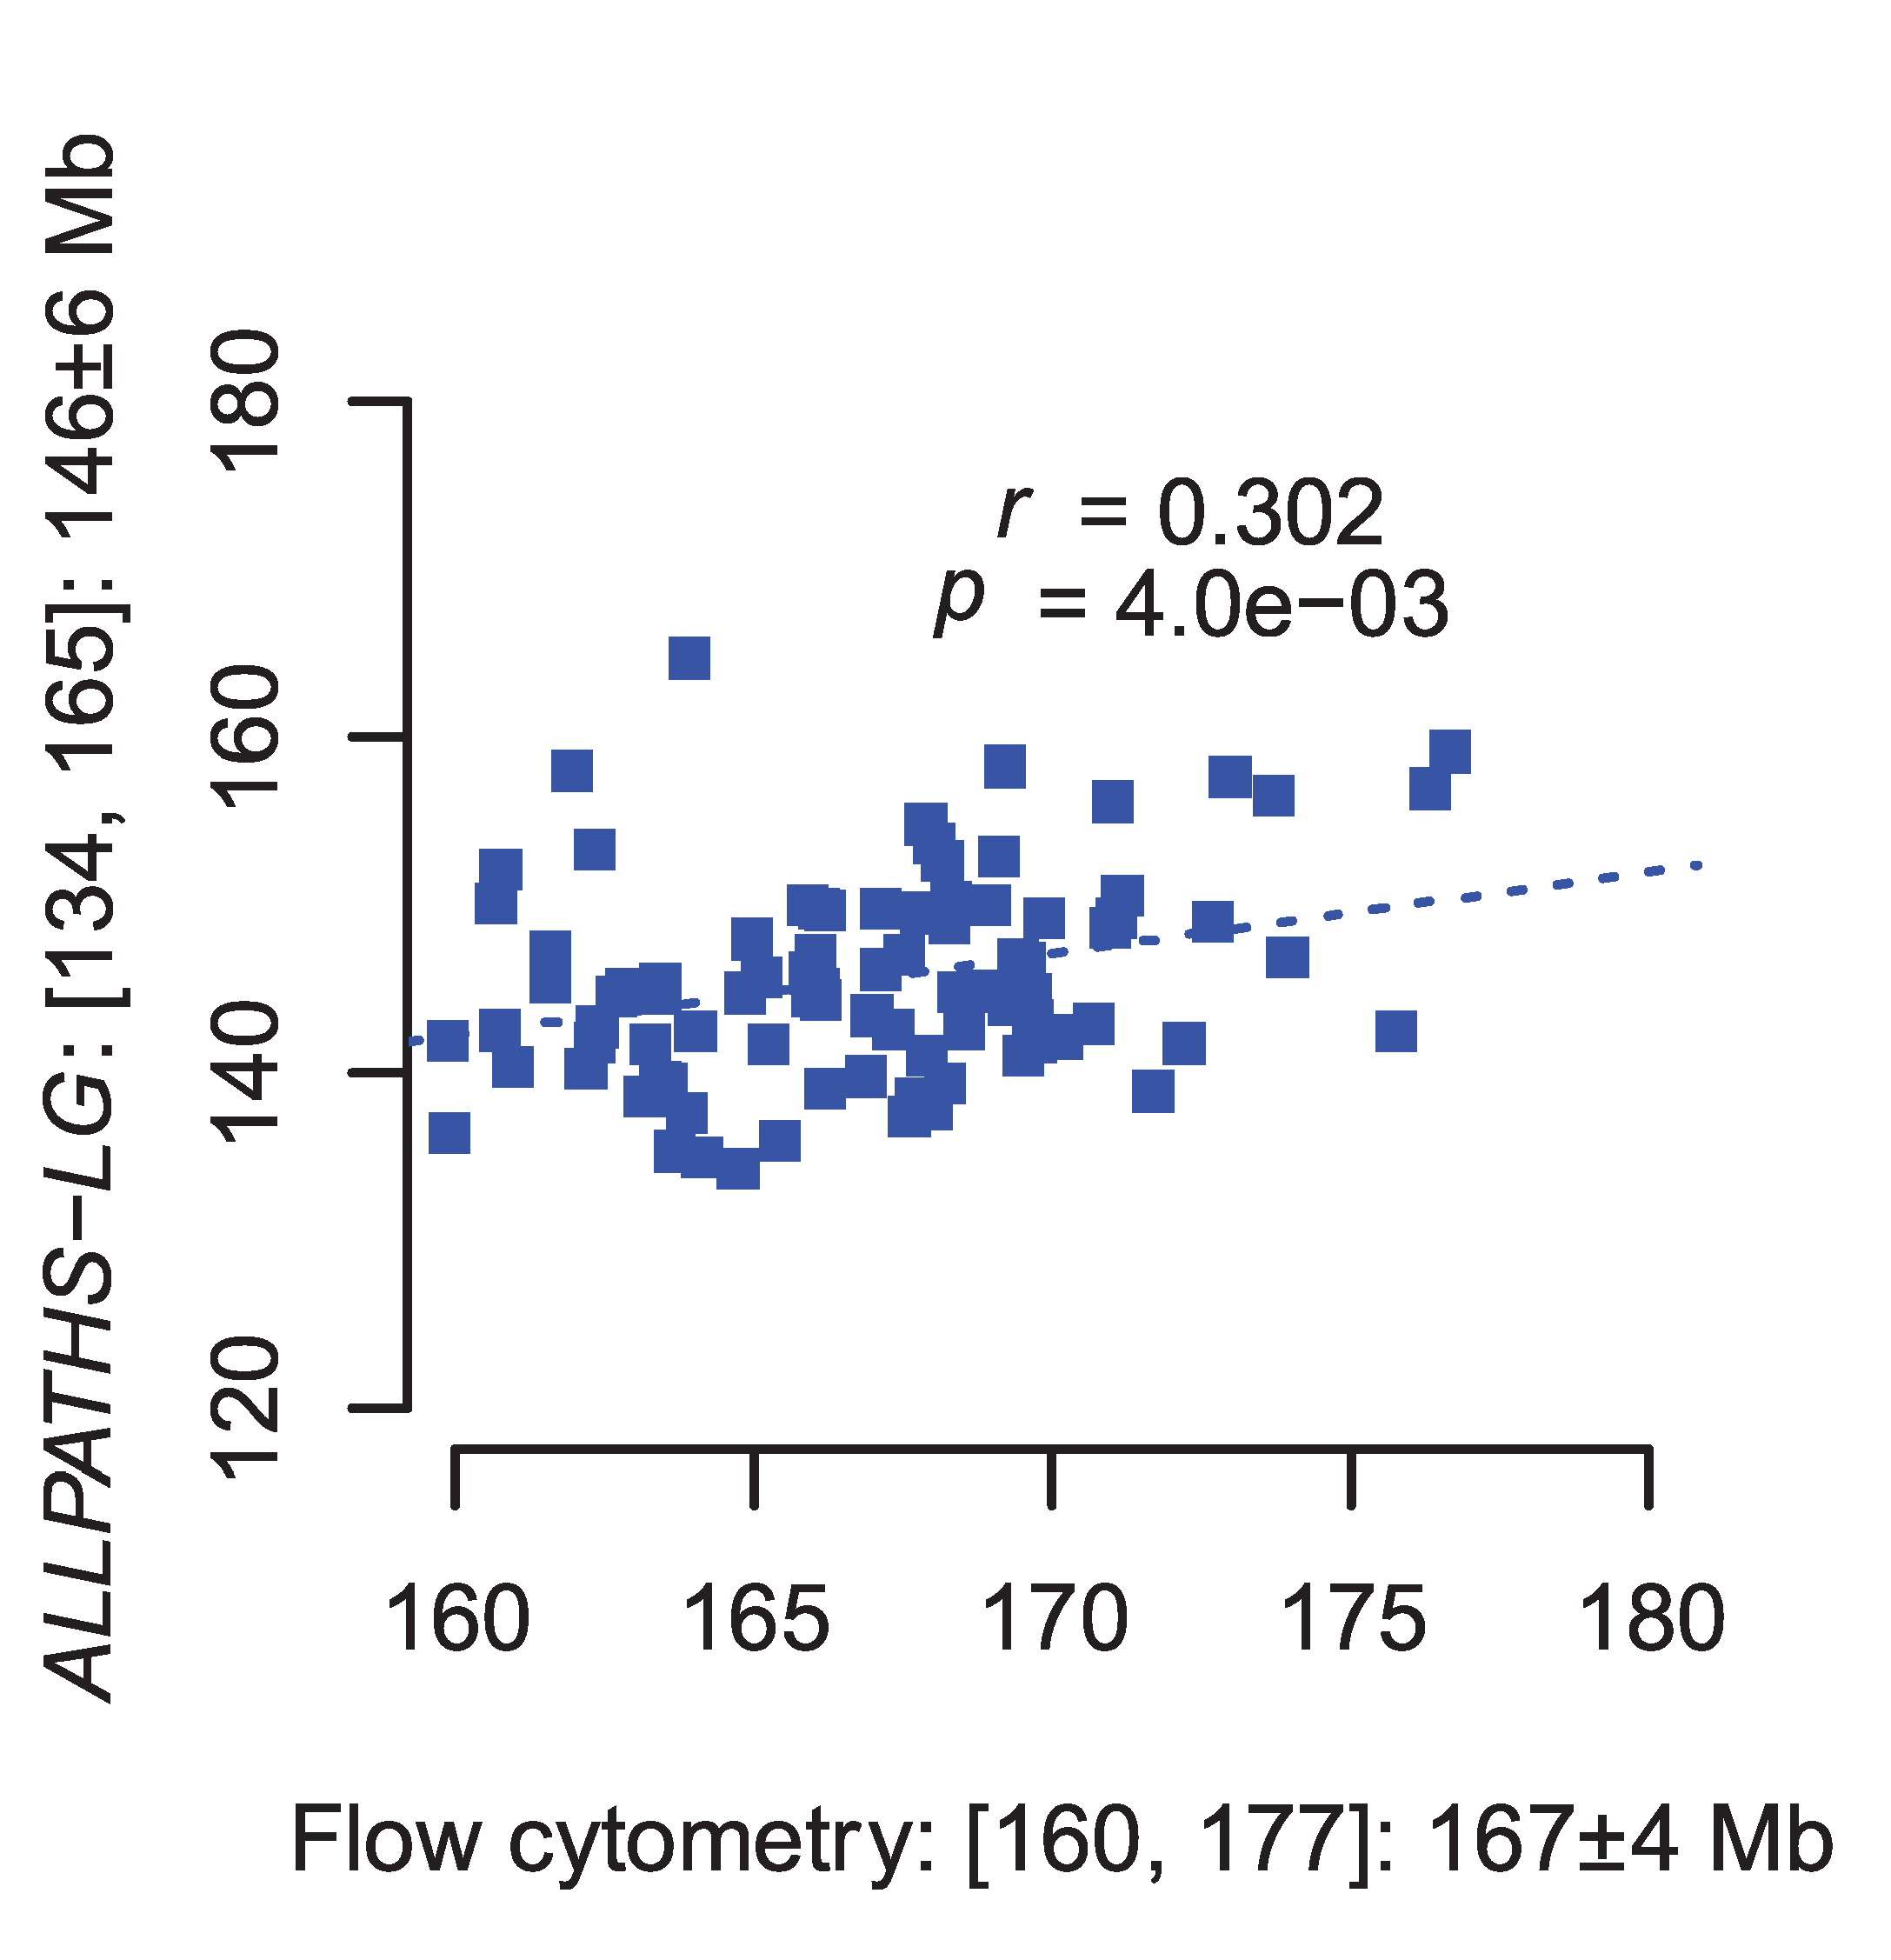
\includegraphics[width=0.37\textwidth]{capitoli/analisi/confronto/confronto1/l.png}} \qquad 
		\subfloat[][\emph{Correlazione tra i valori stimati da findGSE e flow cytometry.}\label{fig:confronto6d}]
			{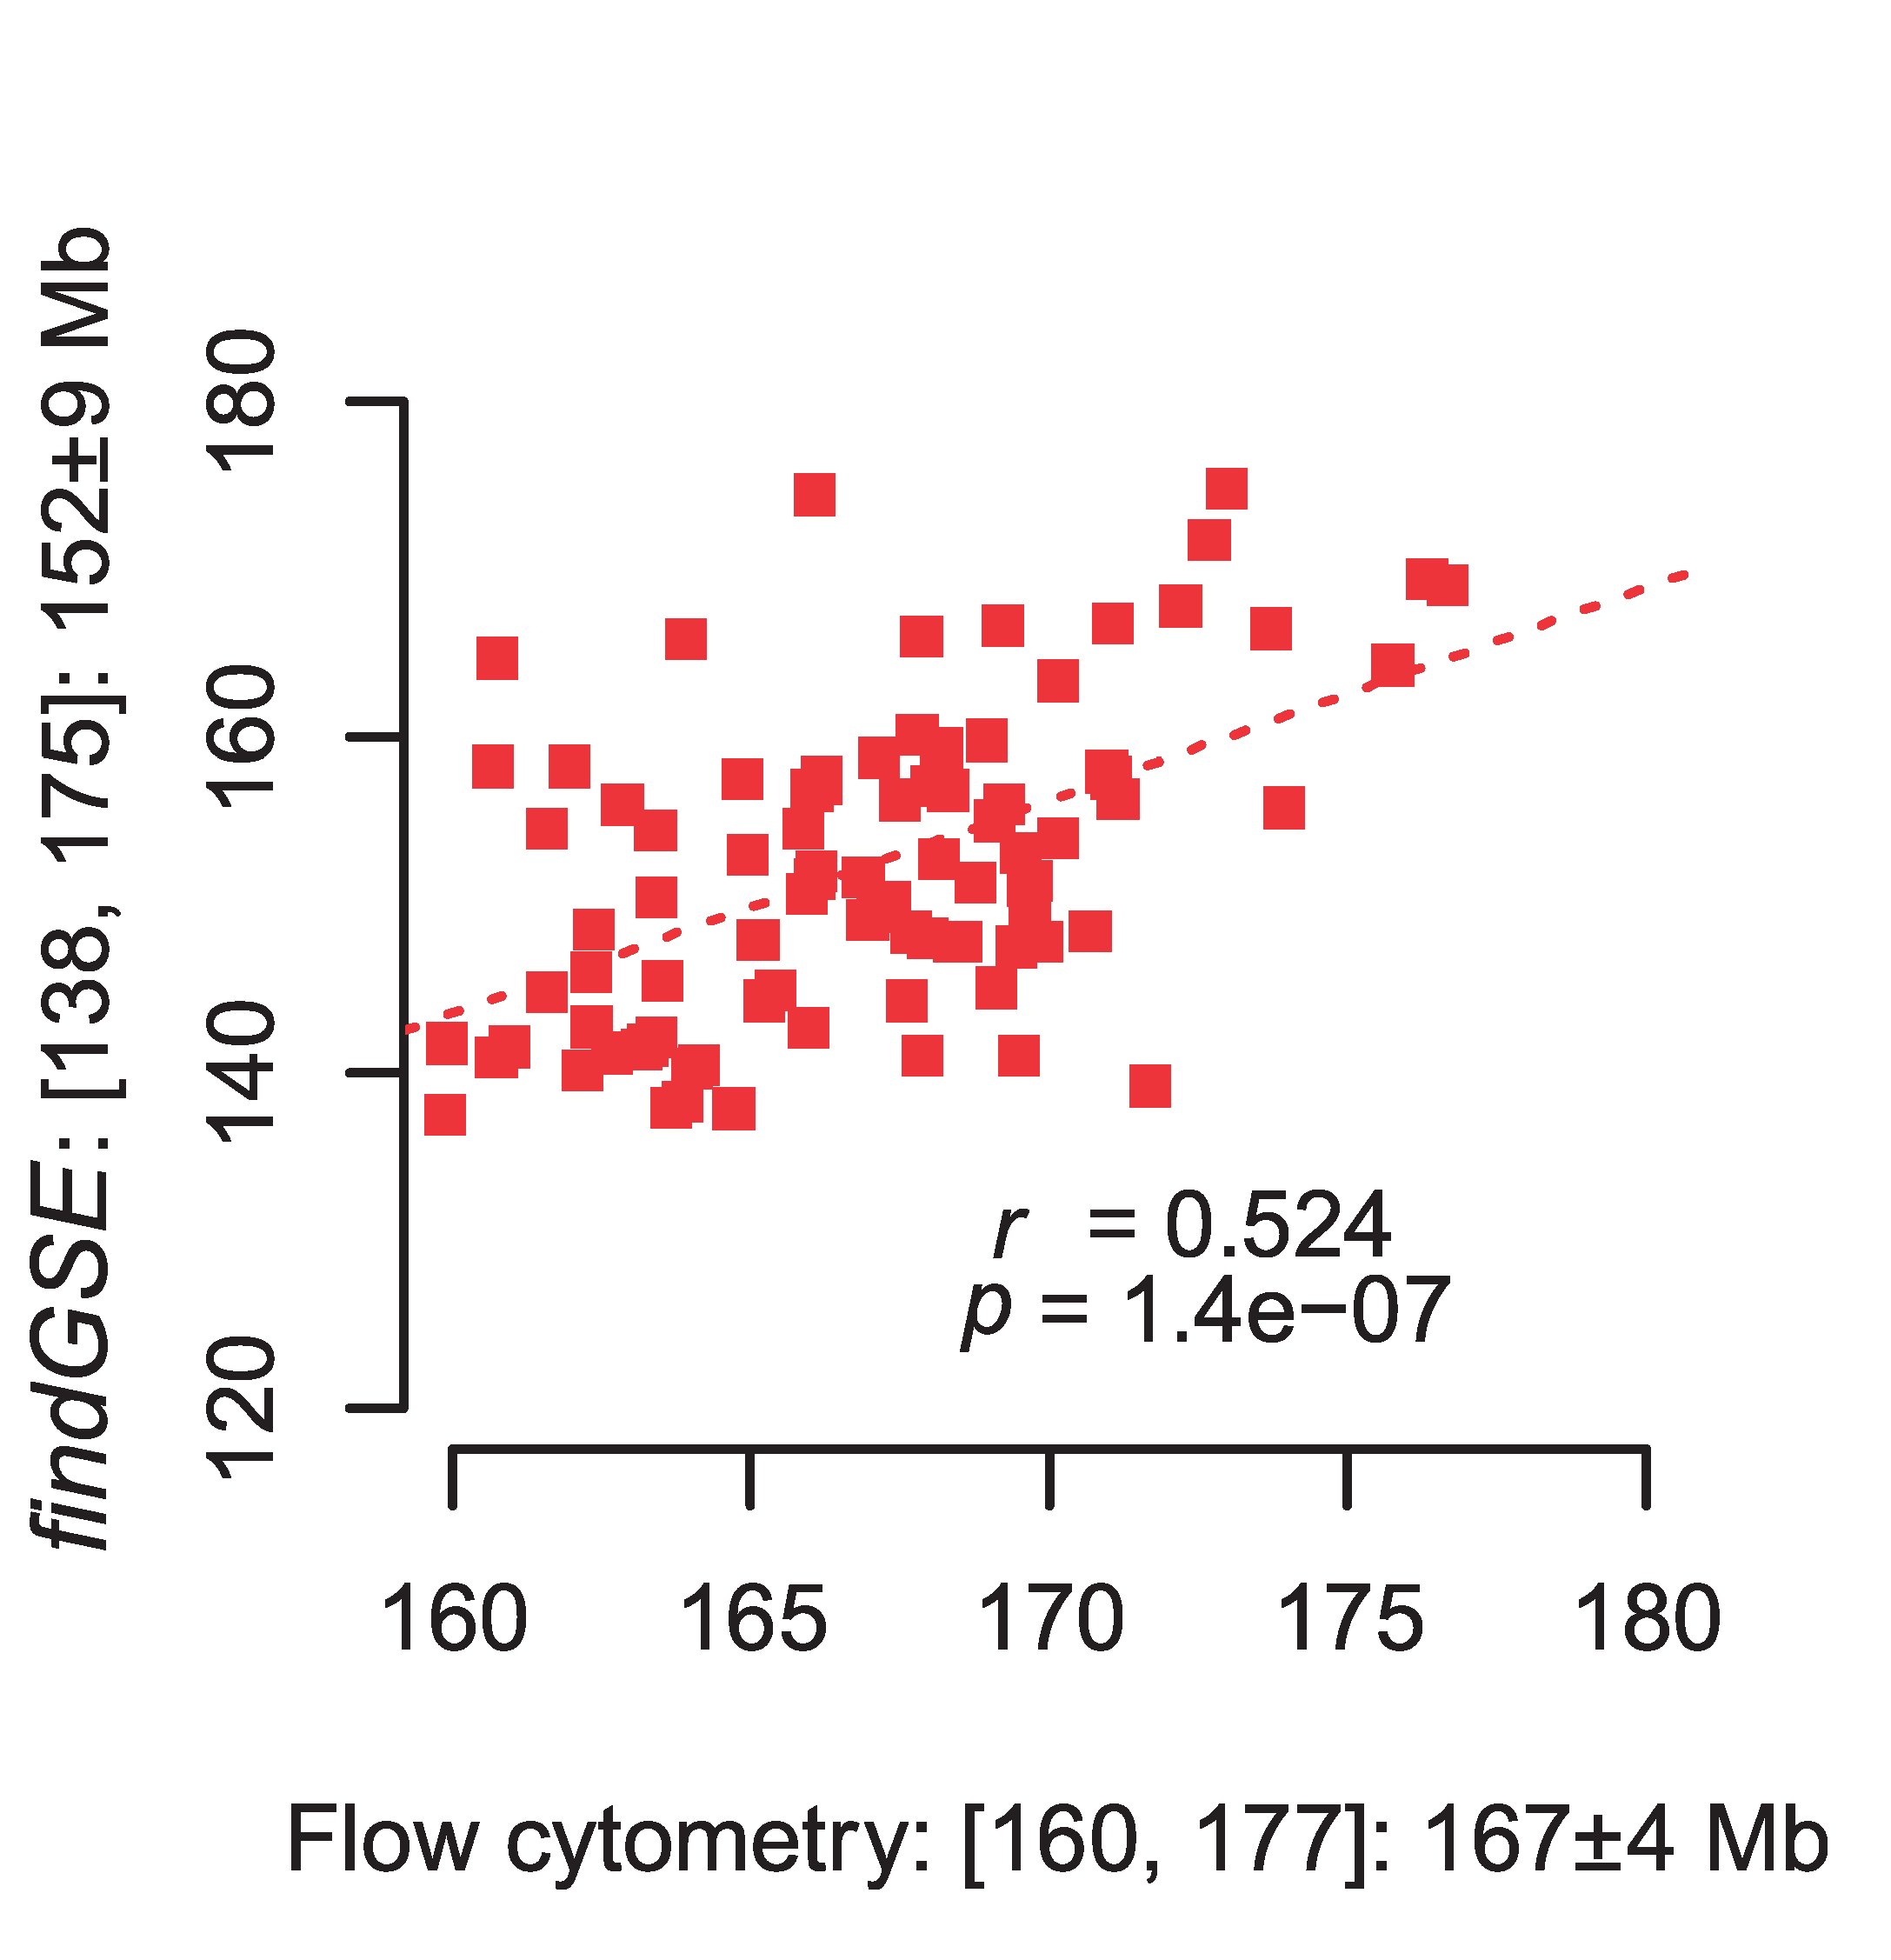
\includegraphics[width=0.37\textwidth]{capitoli/analisi/confronto/confronto1/m.png}} 
		\caption{Correlazione tra i metodi analizzati e flow cytometry. In ciascuna figura sono raffigurate anche la regressione lineare e il \gls{pcc} $r$.}
		\label{fig:confronto6}
	\end{figure}

\end{document}